% Locally compilable (llncs) rendering of the LeafLens manuscript.
% Submission source is paper/main.tex (Springer Nature sn-jnl class).
% Content, numbers, tables and figures are identical; only the document class
% and title-page macros differ so this builds without Springer's proprietary class.
\documentclass[runningheads]{llncs}
\usepackage[T1]{fontenc}
\usepackage{graphicx}
\usepackage{booktabs}
\usepackage{amsmath}
\usepackage{url}
\usepackage{xcolor}
\renewcommand\UrlFont{\color{blue}\rmfamily}
\urlstyle{rm}
\begin{document}
\title{A Physics-Informed Machine Learning Framework for Predicting Gas Exchange in CRISPR Stomatal-Engineered Rice}
\titlerunning{Physics-Informed ML for Stomatal Engineering in Rice}
\author{P. Thrishna Sai\inst{1} \and N. Jenika\inst{1}}
\authorrunning{P. Thrishna Sai, N. Jenika}
\institute{Centre for Biotechnology, Jawaharlal Nehru Technological University Hyderabad --
University College of Engineering Science and Technology Hyderabad (JNTUH-UCESTH),
Hyderabad, Telangana, India\\
\email{thrishnapatlolla1@gmail.com, jenika.nethala@gmail.com}}
\maketitle
\begin{abstract}
CRISPR-Cas9 editing of stomatal-patterning genes can reduce stomatal density and cut transpirational water loss in rice, but choosing how much reduction is appropriate requires a quantitative model of the resulting carbon--water trade-off, and published stomatal-engineering datasets are small. We assembled a harmonized 165-measurement dataset from three published rice studies (Caine et al. 2019; Karavolias et al. 2023, 2024) spanning three cultivars, three gene targets and 14 genotype lines, and developed a physics-informed model that adds a ridge-regression residual to a light-response saturation prior, $y = y_{\max}\,\mathrm{PPFD}/(\mathrm{PPFD}+K_m)\cdot S^{\beta}$, where $S$ is stomatal density relative to wild type. Under genotype-grouped cross-validation repeated across 20 randomized fold assignments, the framework predicts carbon assimilation with $R^{2}=0.53\pm0.17$ and stomatal conductance with $R^{2}=0.36\pm0.15$. The physics prior provides a reproducible benefit over an otherwise identical model without it, improving $R^{2}$ by $+0.116\pm0.091$ for assimilation and $+0.042\pm0.023$ for conductance, and winning in 20 of 20 paired repeats for both targets. We introduce a variance-decomposition diagnostic -- the one-way random-effects intraclass correlation, which correctly discounts singleton replicate cells rather than letting them appear trivially "perfectly explained" -- that establishes the maximum $R^{2}$ any genotype-level predictor can attain given replicate scatter, and use it to show that intrinsic water-use efficiency ($A/g_s$), the target adopted by most comparable analyses including our own earlier work, has a ceiling of $R^{2}=0.00$: after accounting for the design's replicate structure it carries no statistically distinguishable between-genotype signal, its replicate noise being 2.7$\times$ its genotype effect. Modelling $A$ and $g_s$ separately recovers a usable framework where the ratio does not. We report three constraints on deployment, each quantified. First, predictive skill is not uniform: leave-one-genotype-out $R^{2}$ correlates negatively with reduction magnitude (Spearman $\rho=-0.50$ for $A$, $-0.58$ for $g_s$), and the most severe genotypes are the worst predicted. Second, absolute values do not transfer across studies, and normalizing to a within-study wild-type control does not rescue transfer (leave-one-study-out $R^{2}=-0.28$ for $A$, $-0.04$ for $g_s$); with only three studies these estimates are themselves unstable. Third, the literature contains a 29.5-point gap in stomatal-density reduction between 28.5\% and 58\%, and the entire 30--70\% decision-relevant band is represented by a single genotype (5 measurements). Within its validated domain the model predicts that a 30\% reduction retains 94.9\% of wild-type assimilation while reducing conductance to 92.0\%.

\keywords{Physics-Informed Machine Learning \and CRISPR-Cas9 \and Stomatal Engineering \and Gas Exchange \and Cross-Validation \and \textit{Oryza sativa}}
\end{abstract}
% ============================================================
\section{Introduction}\label{sec:intro}

Rice (\textit{Oryza sativa}) supplies more than 20\% of global caloric intake~\cite{ref_fao}, and climate projections indicate that rising temperatures and more frequent droughts will reduce yields in major growing regions~\cite{ref_ipcc}. In Telangana, India, pre-monsoon air temperatures regularly exceed $40\,^{\circ}$C and vapor pressure deficit (VPD) is high, driving transpirational water loss through leaf stomata. Conventional breeding for drought tolerance is slow and bounded by existing genetic variation~\cite{ref_crispr_review}, which motivates direct genetic modification of the traits governing plant water use.

Stomata are pores that mediate the exchange of CO$_2$ and water vapor. Opening them to admit CO$_2$ for photosynthesis necessarily permits water vapor to escape, and this trade-off governs plant carbon gain and water loss. Stomatal density is controlled during leaf development by the Epidermal Patterning Factor (\textit{EPF/EPFL}) peptide family~\cite{ref_hepworth}. Caine et al. (2019) showed that \textit{OsEPF1} overexpression in IR64 rice reduced stomatal density and improved water conservation~\cite{ref_caine}. Karavolias et al. (2023) compared \textit{OsEPFL10} and \textit{OsSTOMAGEN} knockouts in Nipponbare across a light-response gradient, finding that moderate \textit{EPFL10}-mediated reductions conserved water without the assimilation penalty of the severe \textit{stomagen} knockout~\cite{ref_kara2023}. Karavolias et al. (2024) generated a graded \textit{OsSTOMAGEN} promoter-edited allelic series in Kitaake spanning roughly 70--120\% of wild-type density~\cite{ref_kara2024}. Collectively these establish that stomatal density is tunable and that the resulting lines differ in gas exchange, but they do not provide a predictive model that maps a proposed density reduction onto its expected carbon and water consequences under specified environmental conditions.

Biophysical models of stomatal conductance such as Ball--Berry~\cite{ref_ball_berry} and Medlyn et al.~\cite{ref_medlyn} predict gas exchange from environmental drivers, but are parameterized for wild-type anatomy and are not calibrated for edited pore density. Purely data-driven machine learning could in principle learn the effects of editing, but the published CRISPR stomatal-engineering literature offers only low hundreds of measurements, since each data point represents months of growth-chamber time. Physics-informed machine learning (PIML) is frequently proposed for exactly this regime: embedding a known physical law as an inductive bias to reduce the data requirement while keeping predictions physically consistent~\cite{ref_karniadakis,ref_willard}. Whether that promise is realized at the sample sizes actually available here, and what must be done to realize it, is the subject of this paper.

We present \textbf{LeafLens}, a physics-informed framework for predicting gas exchange in stomatal-engineered rice. Our contributions are:

\begin{enumerate}
    \item A harmonized, reproducible 165-measurement dataset from three peer-reviewed CRISPR stomatal-engineering studies, in which every value is traceable to a digitized figure point, a reported genotype mean, or an explicitly flagged regression estimate.
    \item A physics-informed architecture coupling a light-response saturation prior with a ridge residual learner, which predicts assimilation at $R^{2}=0.53\pm0.17$ and conductance at $R^{2}=0.37\pm0.15$ under genotype-grouped cross-validation, and in which the physics prior yields a reproducible benefit (20/20 paired repeats for both targets).
    \item A variance-decomposition diagnostic (a one-way ANOVA intraclass correlation, which correctly discounts singleton-replicate cells) that bounds the maximum attainable $R^{2}$ for any candidate target before modelling, and its application to show that intrinsic water-use efficiency carries no learnable signal in this class of data ($R^{2}$ ceiling $=0.00$) while its two constituent measurements do ($0.830$ and $0.501$).
    \item A quantified account of three deployment constraints: predictive skill declines systematically with the magnitude of the engineered reduction; cross-study transfer fails and is \emph{not} rescued by within-study wild-type normalization; and the decision-relevant 30--70\% reduction band is represented in the entire published literature by a single genotype.
\end{enumerate}

% ============================================================
\section{Related Work}\label{sec:related}

\textbf{Stomatal engineering in crops.} The EPF/EPFL family controls stomatal development across grasses~\cite{ref_hepworth}. The three studies compiled here~\cite{ref_caine,ref_kara2023,ref_kara2024} each use a distinct cultivar, gene target and environmental protocol. That heterogeneity is what makes cross-study synthesis valuable, and also what makes it difficult: within any single study the environmental covariates are held fixed, so environment and study identity are confounded by design.

\textbf{Stomatal conductance models.} Ball--Berry~\cite{ref_ball_berry} and Medlyn et al.~\cite{ref_medlyn} relate conductance to assimilation, CO$_2$ and humidity or VPD. These are wild-type calibrations and are not expected to hold once pore density is edited, which is the gap a learned residual is intended to close. For the light dependence of assimilation we instead adopt a saturating light-response form, which is standard in photosynthesis physiology and, as we show, is a far better-behaved prior than an uncalibrated water-use-efficiency heuristic.

\textbf{PIML and small-sample validation.} PIML embeds physical laws into learning pipelines through loss terms, architecture or features~\cite{ref_karniadakis,ref_willard}. Its behaviour in the very-small-sample, multi-source regime typical of plant gene-editing data is less well characterized, and validation design is critical there: with a handful of genotypes, a shuffled cross-validation split routinely places replicate measurements of the same genotype in both training and test folds, inflating $R^{2}$ without demonstrating generalization to a new genotype. ML has been applied broadly in agriculture to yield prediction, disease detection and irrigation scheduling~\cite{ref_ml_agri}; we are not aware of prior work applying PIML to CRISPR stomatal engineering with genotype-grouped validation.

% ============================================================
\section{Materials and Methods}\label{sec:methods}

Figure~\ref{fig:pipeline} summarizes the pipeline: digitized gas-exchange measurements and satellite climate records feed a hybrid model combining a biophysical prior with a learned residual, which is evaluated under genotype-grouped and leave-one-study-out cross-validation.

\begin{figure}[t]
\centering
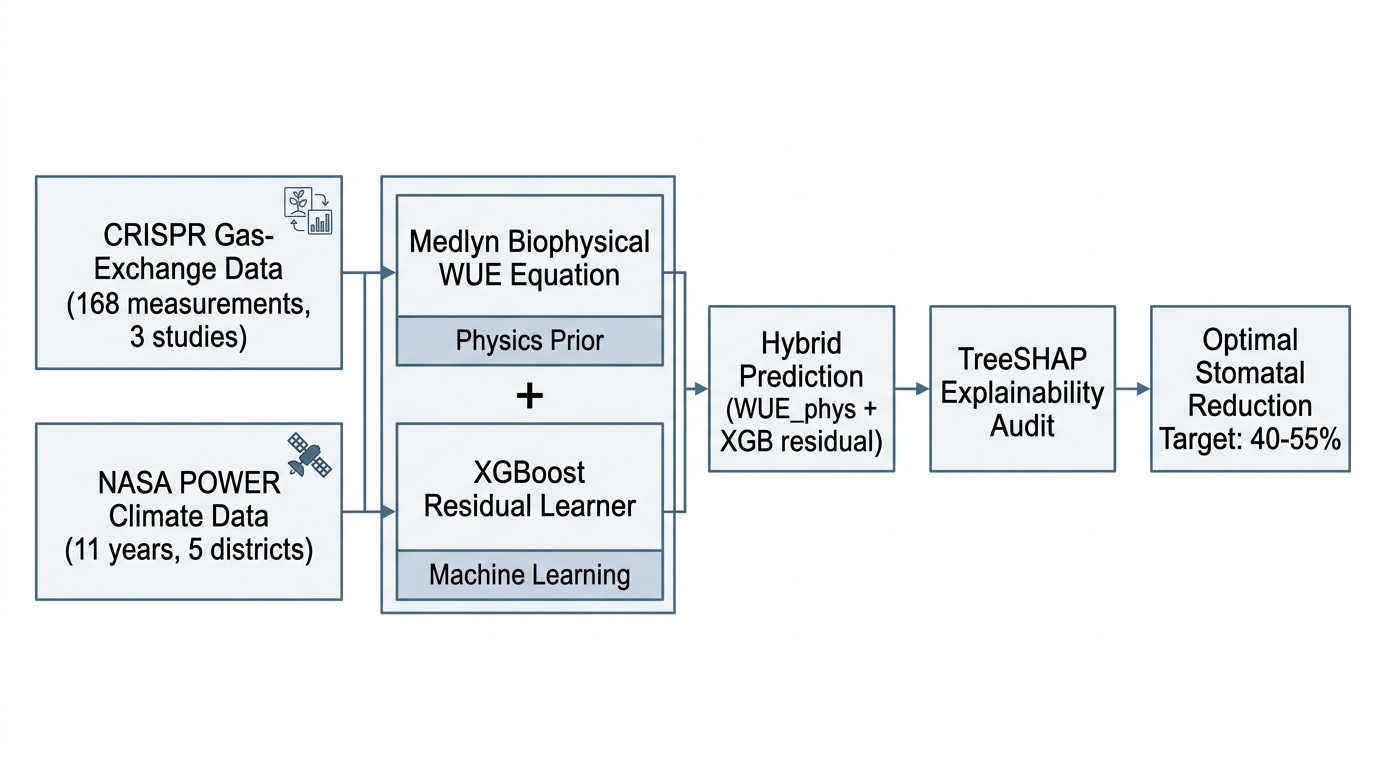
\includegraphics[width=\textwidth]{figures/fig_pipeline.jpg}
\caption{Overview of the LeafLens framework. CRISPR gas-exchange data and NASA POWER climate data feed a physics-informed model whose predictions are validated on held-out genotypes and held-out studies before any climate application.}
\label{fig:pipeline}
\end{figure}

\subsection{Experimental Data Compilation}\label{sec:data}

We compiled gas-exchange data from three published studies. Values not stated numerically in the source text were digitized from published figures with WebPlotDigitizer. After harmonization and removal of three duplicate records, the dataset comprises \textbf{165 measurements} across 14 genotype lines, three cultivars and three gene targets (Table~\ref{tab:dataset}): 106 well-watered and 59 drought-treated. We count 14 rather than 12 lines because the \textit{stomagen} knockout and the wild-type control each appear in two studies in different cultivar backgrounds (Nipponbare and Kitaake), and are biologically distinct lines despite sharing a name.

\begin{table}[t]
\caption{Compiled CRISPR rice stomatal-engineering dataset.}\label{tab:dataset}
\centering
\small
\begin{tabular}{lllcp{3.4cm}}
\toprule
\textbf{Study} & \textbf{Gene / Edit} & \textbf{Cultivar} & \textbf{$n$} & \textbf{Conditions} \\
\midrule
Caine et al. (2019) & \textit{OsEPF1} OE & IR64 & 15 & PAR 1000, $T{=}30\,^\circ$C, well-watered \\
Karavolias et al. (2023) & \textit{OsEPFL10}/\textit{OsSTOMAGEN} KO & Nipponbare & 30 & PAR 50--2000, $T{=}28\,^\circ$C, well-watered \\
Karavolias et al. (2024) & \textit{OsSTOMAGEN} promoter & Kitaake & 120 & PAR 1500, $T{=}29/31\,^\circ$C, watered \& drought \\
\midrule
\textbf{Total} & \textbf{3 gene targets} & \textbf{3 cultivars} & \textbf{165} & \\
\bottomrule
\end{tabular}
\end{table}

Two Karavolias et al. (2024) promoter alleles (Alleles 5 and 6) carry \emph{higher} stomatal density than wild type; this is a genuine hypermorphic phenotype reported by that study and both are retained. For Caine et al. (2019) we take the stomatal-density reductions directly from that paper's Results text (58\% for \textit{OsEPF1oe}W and 88\% for \textit{OsEPF1oe}S relative to IR64 controls), since only the ratio to wild type enters the model. Assimilation values for the Karavolias et al. (2024) well-watered cohort are the per-genotype means reported in that study's Fig.~2B. No paired assimilation measurement exists for its drought cohort, where only conductance is reported; for those 59 rows we estimate $A$ from measured drought $g_s$ using the linear relationship $A = 45.74\,g_s + 6.12$ fitted on the study's own steady-state genotype means ($R^{2}=0.931$, $n=8$). Every such value is flagged in the released dataset (\texttt{A\_Source}) and the consequences are addressed in Section~\ref{sec:limitations}. Figure~\ref{fig:scatter_a_gs} shows the raw relationships between stomatal reduction and both gas-exchange variables.

\begin{figure}[t]
\centering
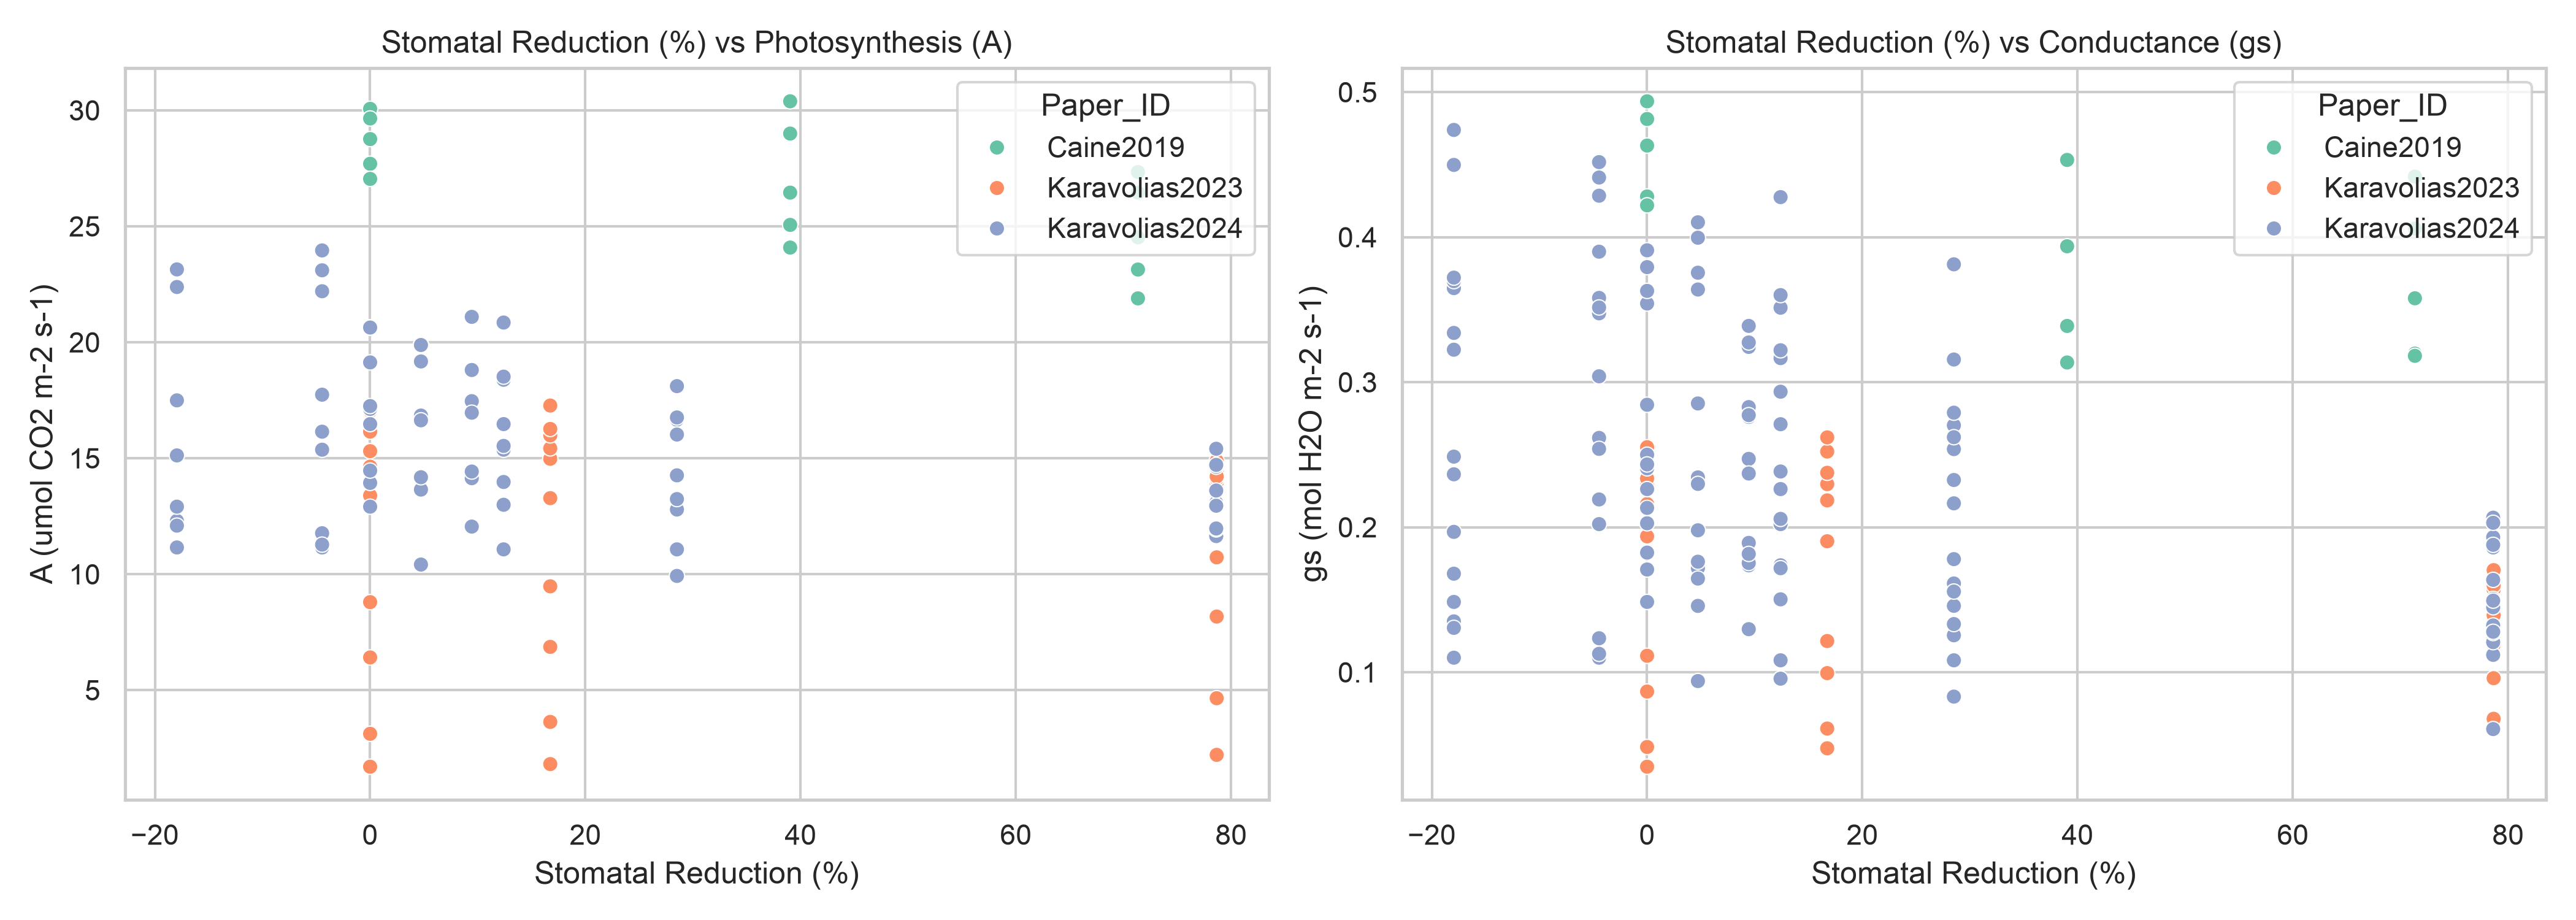
\includegraphics[width=\textwidth]{figures/fig_scatter_a_gs.png}
\caption{Raw data from the three studies. \textbf{Left:} assimilation ($A$) versus stomatal density reduction. \textbf{Right:} conductance ($g_s$) versus reduction. Colors indicate study.}
\label{fig:scatter_a_gs}
\end{figure}

\subsection{Regional Climate Data}\label{sec:climate}

We retrieved 11.5 years (January 2015--June 2026) of daily NASA POWER data~\cite{ref_nasa} for five Telangana districts (Warangal, Nizamabad, Karimnagar, Nalgonda, Khammam). VPD was computed from daily temperature and relative humidity using the Tetens/Murray saturation-vapor-pressure form as given in Allen et al.~\cite{ref_fao56}:
\begin{equation}
e_s(T) = 0.6108 \exp\!\Bigl(\frac{17.27\,T}{T + 237.3}\Bigr),\qquad
\mathrm{VPD} = e_s(T)\Bigl(1 - \tfrac{\mathrm{RH}}{100}\Bigr).
\end{equation}
Photosynthetic photon flux density was derived from daily shortwave irradiance as $\mathrm{PPFD} = R_s\times10^{6}\times f_{\mathrm{PAR}}\times q / D$, with PAR fraction $f_{\mathrm{PAR}}=0.45$~\cite{ref_mccree}, quantum conversion $q=4.6\,\mu$mol\,J$^{-1}$, and assumed photoperiod $D=43\,200$\,s, giving a daytime-average PPFD of 51--1351\,$\mu$mol\,m$^{-2}$\,s$^{-1}$. Figure~\ref{fig:vpd} shows the monthly VPD distribution, which peaks in April--May with district-seasonal means up to 3.39\,kPa.

\begin{figure}[t]
\centering
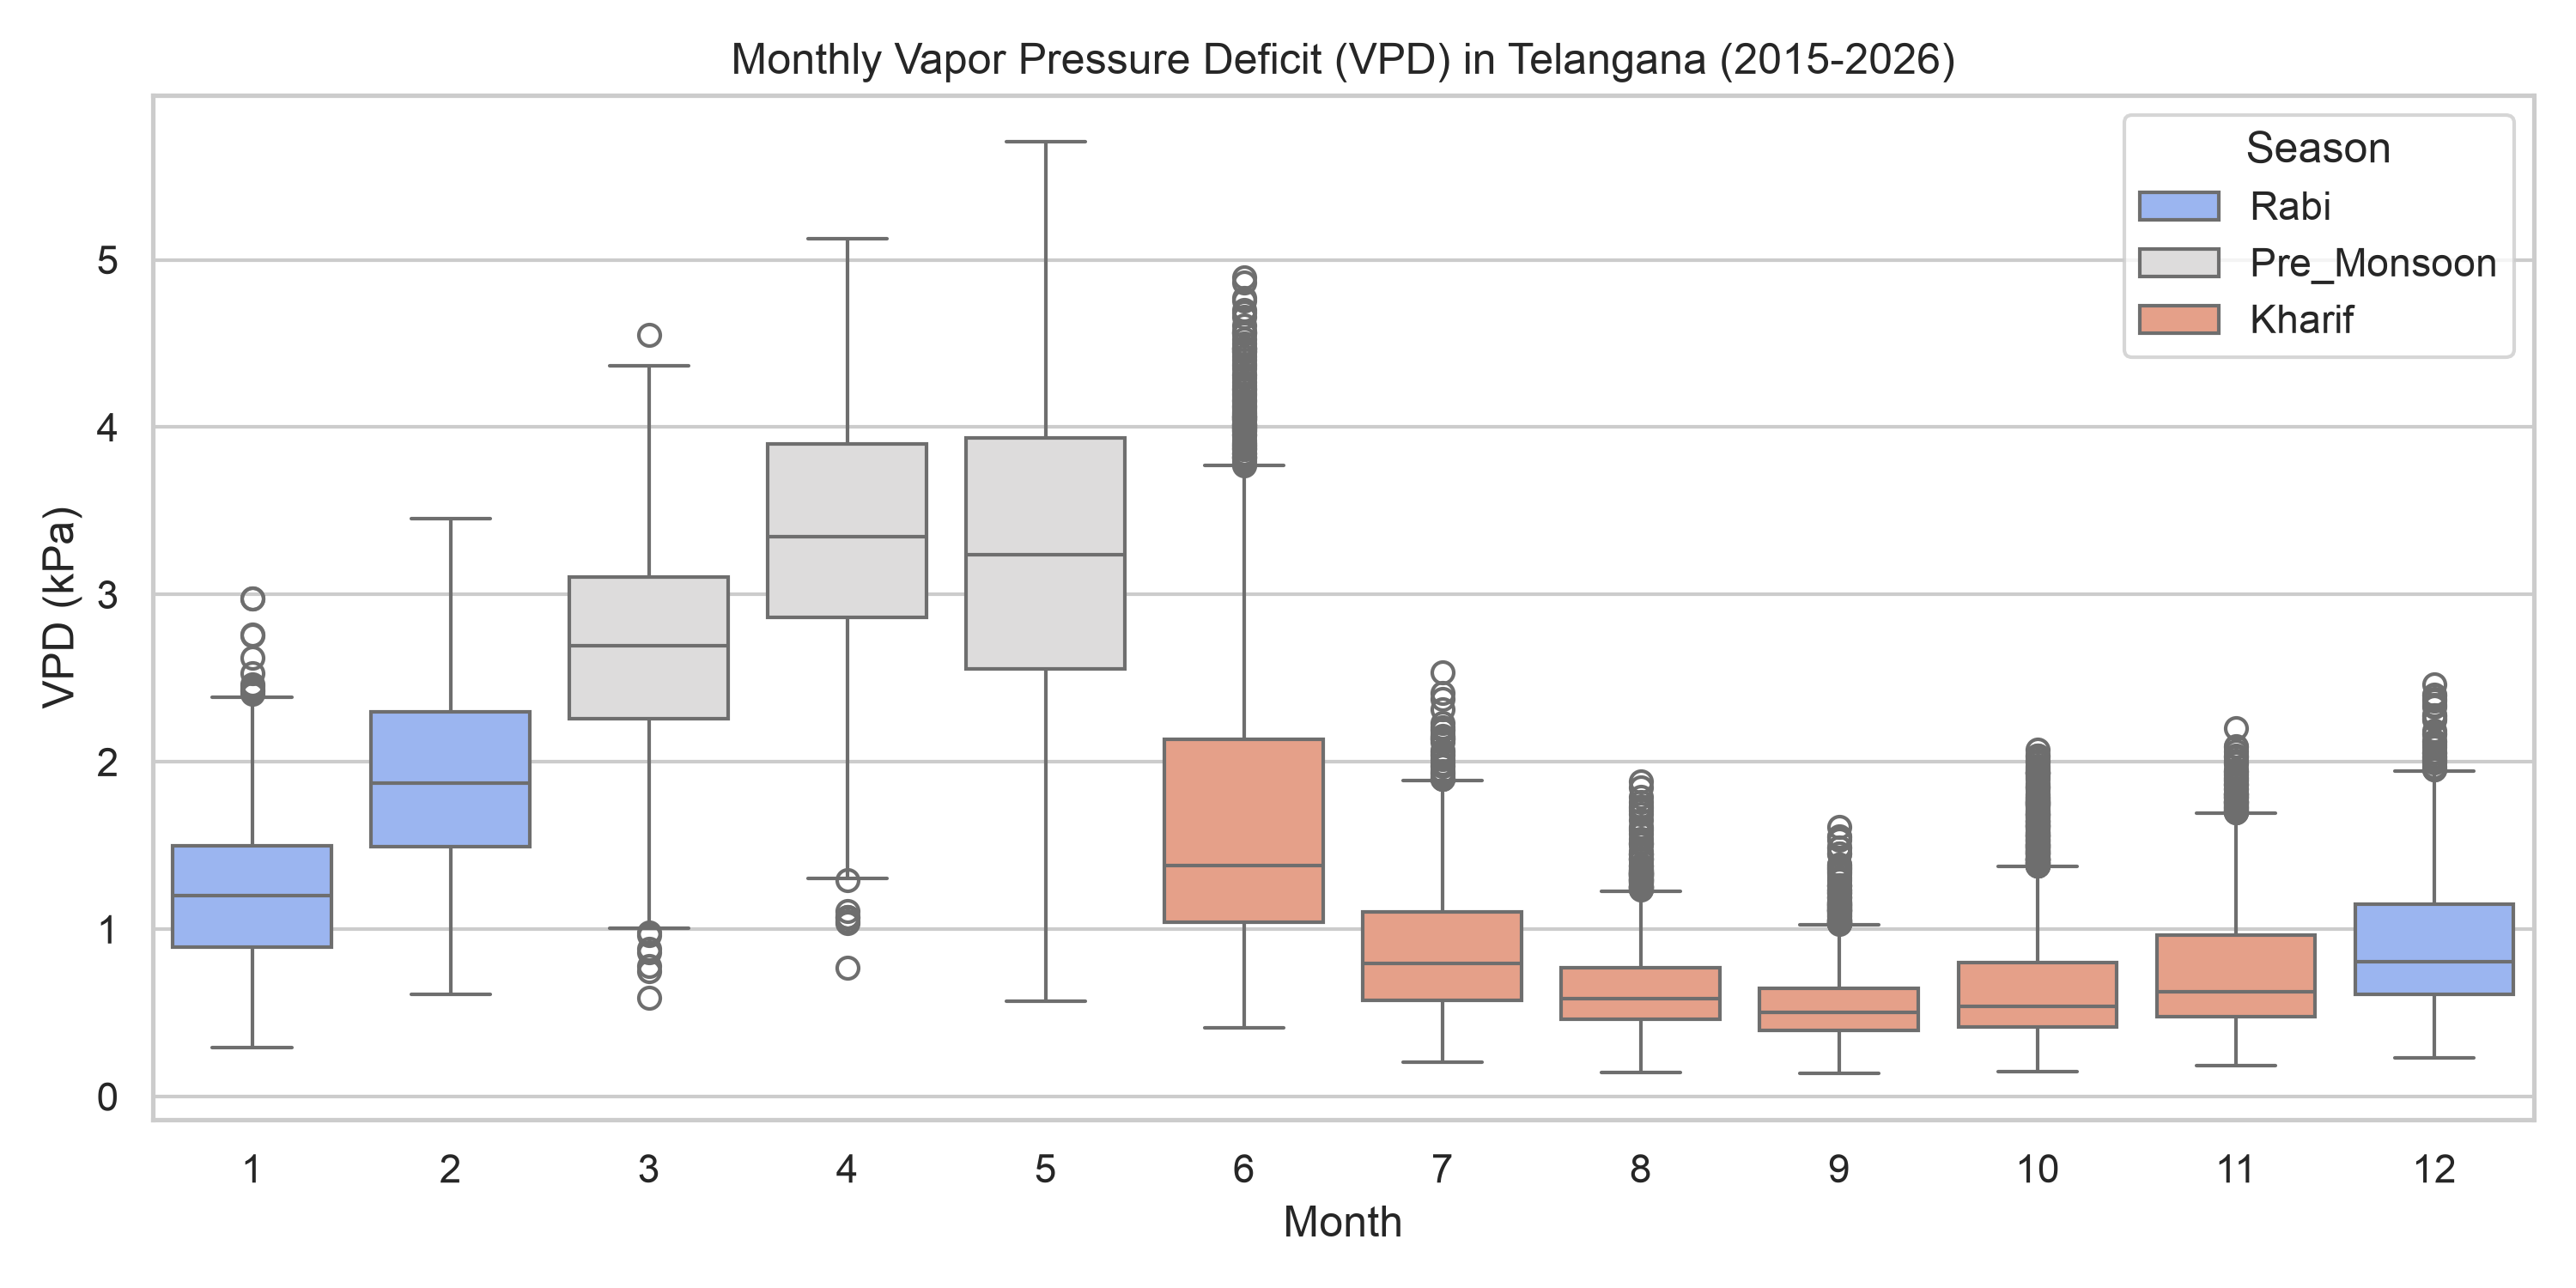
\includegraphics[width=\textwidth]{figures/fig_vpd_monthly.png}
\caption{Monthly VPD across five Telangana districts (2015--2026), colored by season. VPD peaks in the April--May pre-monsoon window.}
\label{fig:vpd}
\end{figure}

\subsection{Target Selection by Variance Decomposition}\label{sec:ceiling}

Before fitting any model we bound what is learnable. A predictor built from genotype and environmental features can only distinguish observations that differ in those features; it cannot resolve replicate scatter among measurements sharing identical values. Partitioning total variance into between-cell and within-cell components, where a cell is one genotype $\times$ study $\times$ water treatment $\times$ light level, bounds the maximum $R^{2}$ attainable by any such predictor. A naive between/total sum-of-squares ratio is not a safe estimator of this bound: 30 of our 49 cells contain a single replicate, and a singleton cell has zero within-cell sum of squares by construction, so it appears "perfectly explained" while carrying no information about replicate noise -- inflating the naive ratio. We instead use the one-way random-effects ANOVA intraclass correlation~\cite{ref_searle}, which lets singleton cells inform the between-group mean while contributing zero degrees of freedom to the within-group error term, the statistically correct treatment:
\begin{equation}\label{eq:ceiling}
R^{2}_{\max} = \mathrm{ICC} = \frac{\hat{\sigma}^{2}_{\text{between}}}{\hat{\sigma}^{2}_{\text{between}} + \hat{\sigma}^{2}_{\text{within}}},
\qquad
\hat{\sigma}^{2}_{\text{between}} = \max\!\left(\frac{\mathrm{MS}_{B}-\mathrm{MS}_{W}}{n_0},\,0\right),
\end{equation}
with $\mathrm{MS}_B$, $\mathrm{MS}_W$ the between- and within-group mean squares and $n_0$ the standard unbalanced-design correction to average group size~\cite{ref_searle}. We compute Eq.~\ref{eq:ceiling} for three candidate targets and select on that basis (Section~\ref{sec:whyceiling}).

\subsection{Physics Prior and Model Architecture}\label{sec:model}

For both targets we use a saturating light-response prior scaled by relative stomatal density:
\begin{equation}\label{eq:phys}
\hat{y}_{\text{phys}} = y_{\max}\,\frac{\mathrm{PPFD}}{\mathrm{PPFD}+K_m}\;S^{\beta},
\qquad S = 1 - \frac{r}{100},
\end{equation}
where $r$ is relative stomatal-density reduction (\%), and $y_{\max}$, $K_m$, $\beta$ are fitted by non-linear least squares on the training fold only. The saturating term is the standard description of light-limited assimilation; the $S^{\beta}$ term expresses supply limitation by pore density, with $\beta$ estimated rather than assumed. A residual learner is then fit on $\varepsilon = y - \hat{y}_{\text{phys}}$ over the feature vector $\mathbf{x} = (S,\ \mathrm{PPFD},\ \mathrm{VPD},\ \mathrm{drought},\ T,\ \mathrm{CO}_2)$, and the prediction is $\hat{y} = \hat{y}_{\text{phys}} + f(\mathbf{x})$.

We use ridge regression ($\alpha=1$) rather than gradient-boosted trees for the residual. Under genotype-grouped validation the model must predict a genotype whose stomatal-density value it has never seen; tree ensembles produce piecewise-constant fits and cannot interpolate across a held-out level of the principal continuous predictor, whereas a linear residual can. We report both in Section~\ref{sec:perf}.

\subsection{Validation Protocol}\label{sec:validation}

A single grouped split is high-variance with only 14 genotype-line groups, so we report genotype-grouped 5-fold cross-validation \emph{repeated over 20 randomized group-to-fold assignments}, quoting the mean and standard deviation of per-fold $R^{2}$. To test whether the physics prior helps, we compare the hybrid against an otherwise identical model without the prior \emph{on identical folds}, and report the paired difference. Leave-one-study-out cross-validation is reported separately as the cross-domain test. Shuffled (ungrouped) cross-validation is reported only to quantify leakage, never as a performance claim.

% ============================================================
\section{Results}\label{sec:results}

\subsection{Which Targets Are Learnable}\label{sec:whyceiling}

Table~\ref{tab:ceiling} applies Eq.~\ref{eq:ceiling} to three candidate targets. Assimilation and conductance are largely learnable; their ratio is not. For intrinsic water-use efficiency the ICC is $0.000$: after correctly discounting singleton-cell replicates, there is no between-genotype variance left to distinguish from noise. The effect size makes the reason concrete: across genotypes, mean $A/g_s$ relative to wild type spans 0.96--1.29 (standard deviation 0.087), while the mean within-genotype replicate standard deviation is 0.238 -- the noise is 2.7$\times$ larger than the entire biological signal. A ratio of two independently noisy measurements compounds the noise of both.

\begin{table}[t]
\caption{Maximum attainable $R^{2}$ for each candidate target, via the ANOVA ICC (Eq.~\ref{eq:ceiling}).}\label{tab:ceiling}
\centering
\small
\begin{tabular}{lcc}
\toprule
\textbf{Target} & \textbf{$R^{2}$ ceiling (ICC)} & \textbf{Irreducible noise} \\
\midrule
$A$ (assimilation) & $0.830$ & $17.0\%$ \\
$g_s$ (conductance) & $0.501$ & $49.9\%$ \\
$A/g_s$ (intrinsic WUE) & $0.000$ & $100\%$ \\
\bottomrule
\end{tabular}
\end{table}

This is confirmed empirically under genotype-grouped validation. Regressing $A/g_s$ directly gives $R^{2}=-0.40\pm1.00$, and deriving it post hoc as the quotient of separately predicted $A$ and $g_s$ is no better ($R^{2}=-0.36\pm0.41$), because the ratio compounds the errors of both components. We therefore model $A$ and $g_s$ separately and present the carbon--water trade-off as a pair of validated predictions rather than a single ratio. Figure~\ref{fig:ceiling} visualizes the decomposition.

\begin{figure}[t]
\centering
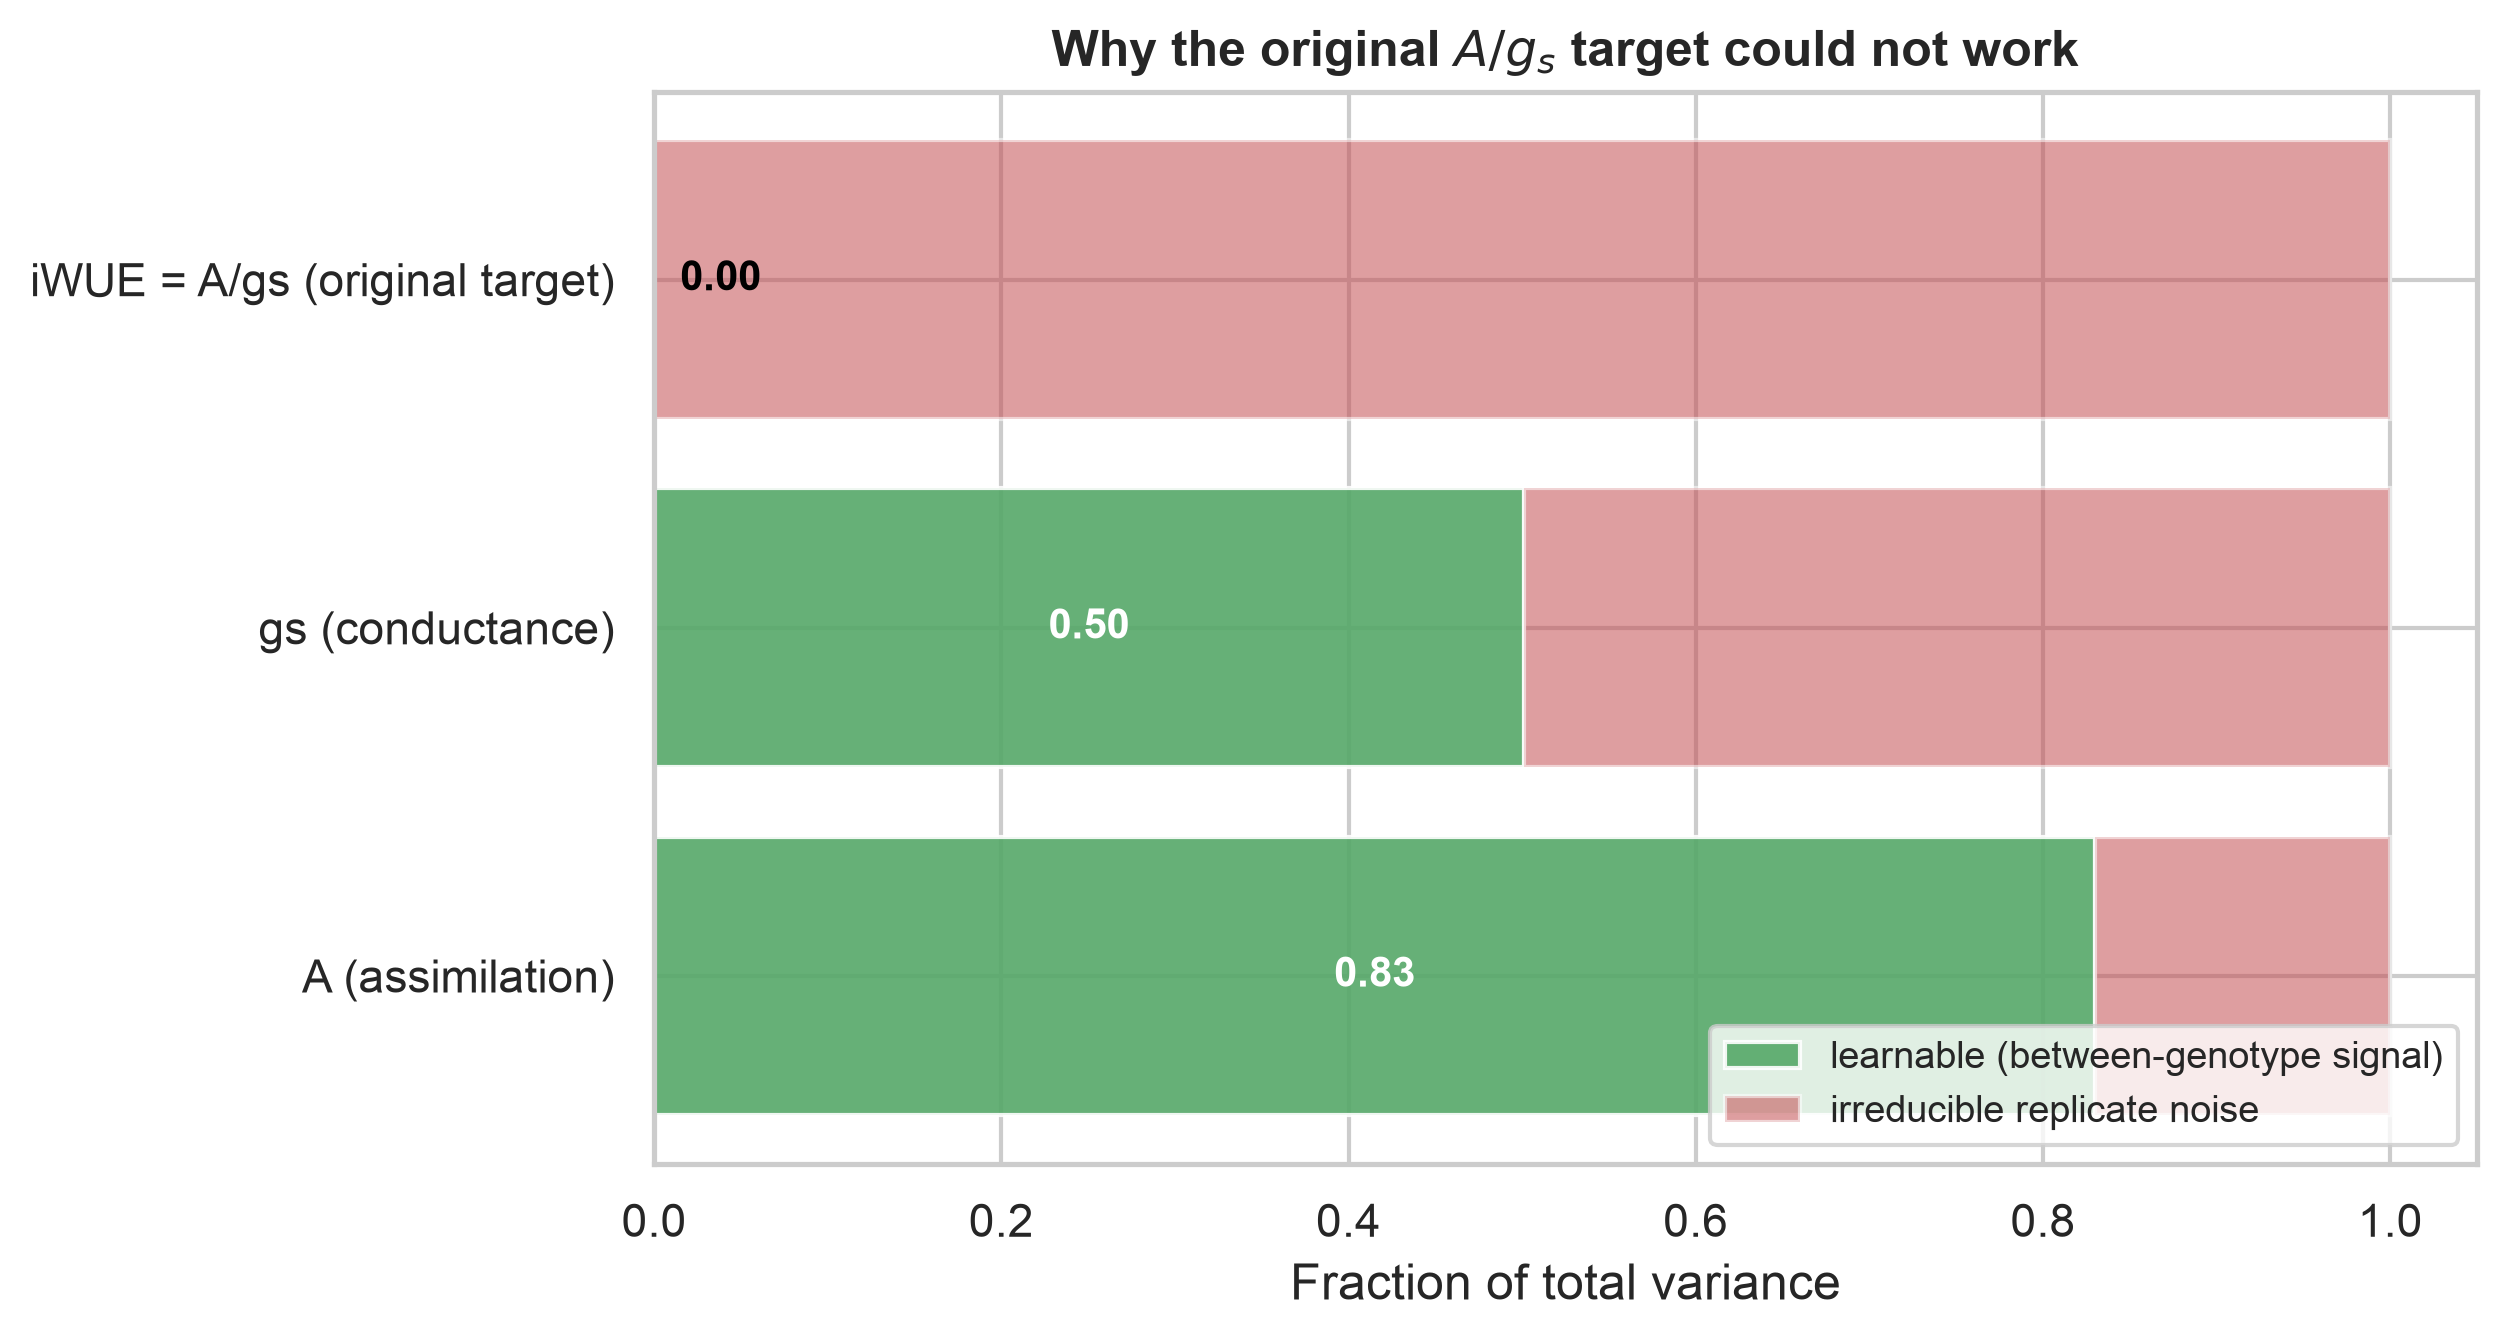
\includegraphics[width=0.8\textwidth]{figures/fig_variance_ceiling.png}
\caption{Variance decomposition for the three candidate targets. Green is the between-genotype signal available to any feature-based predictor; red is irreducible replicate scatter. The $A/g_s$ ratio retains almost no learnable signal.}
\label{fig:ceiling}
\end{figure}

\subsection{Predictive Performance}\label{sec:perf}

Table~\ref{tab:perf} reports genotype-grouped cross-validation across 20 randomized fold assignments. The physics-informed hybrid with a ridge residual is the best model for both targets, reaching $R^{2}=0.531\pm0.166$ for assimilation (64\% of the attainable ceiling) and $R^{2}=0.362\pm0.152$ for conductance (72\% of ceiling).

\begin{table}[t]
\caption{Genotype-grouped CV $R^{2}$ (mean $\pm$ s.d. over 20 randomized fold assignments).}\label{tab:perf}
\centering
\small
\begin{tabular}{lcccc}
\toprule
& \multicolumn{2}{c}{\textbf{$A$ (ICC ceiling 0.830)}} & \multicolumn{2}{c}{\textbf{$g_s$ (ICC ceiling 0.501)}} \\
\cmidrule(lr){2-3}\cmidrule(lr){4-5}
\textbf{Model} & $R^{2}$ & \% of ceiling & $R^{2}$ & \% of ceiling \\
\midrule
Pure physics law (no ML) & $-0.860\pm1.990$ & --- & $-0.517\pm0.809$ & --- \\
Naive ML (XGBoost, no physics) & $-0.060\pm1.213$ & --- & $-0.335\pm0.664$ & --- \\
Physics-informed hybrid (XGB residual) & $0.004\pm1.410$ & 0\% & $-0.204\pm0.648$ & --- \\
Naive ML (Ridge, no physics) & $0.415\pm0.235$ & 50\% & $0.320\pm0.161$ & 64\% \\
\textbf{Physics-informed hybrid (Ridge)} & $\mathbf{0.531\pm0.166}$ & \textbf{64\%} & $\mathbf{0.362\pm0.152}$ & \textbf{72\%} \\
\bottomrule
\end{tabular}
\end{table}

Two patterns are consistent across both targets. First, the physics prior alone is a poor predictor but a useful bias: applied without a residual learner it scores below zero, yet adding it to a learner improves that learner. Second, model class matters more than is usually assumed at this sample size -- every tree-based variant is both worse and far less stable (standard deviations up to 0.78) than its ridge counterpart, consistent with the inability of piecewise-constant fits to interpolate to a held-out genotype's density value.

The paired comparison isolates the contribution of the prior on identical folds (Table~\ref{tab:paired}). The physics prior improves $R^{2}$ by $+0.116\pm0.091$ for assimilation and $+0.042\pm0.023$ for conductance, and wins in 20 of 20 repeats for both targets, so the benefit is reproducible rather than an artifact of a favourable split. Figure~\ref{fig:modelperf} shows all variants against their ceilings, and Figure~\ref{fig:predobs} shows out-of-fold predictions against observations.

\begin{table}[t]
\caption{Paired benefit of the physics prior, evaluated on identical folds.}\label{tab:paired}
\centering
\small
\begin{tabular}{lccc}
\toprule
\textbf{Target} & \textbf{Mean $\Delta R^{2}$} & \textbf{s.d.} & \textbf{Repeats won} \\
\midrule
$A$ (assimilation) & $+0.116$ & $0.091$ & 20/20 \\
$g_s$ (conductance) & $+0.042$ & $0.023$ & 20/20 \\
\bottomrule
\end{tabular}
\end{table}

\begin{figure}[t]
\centering
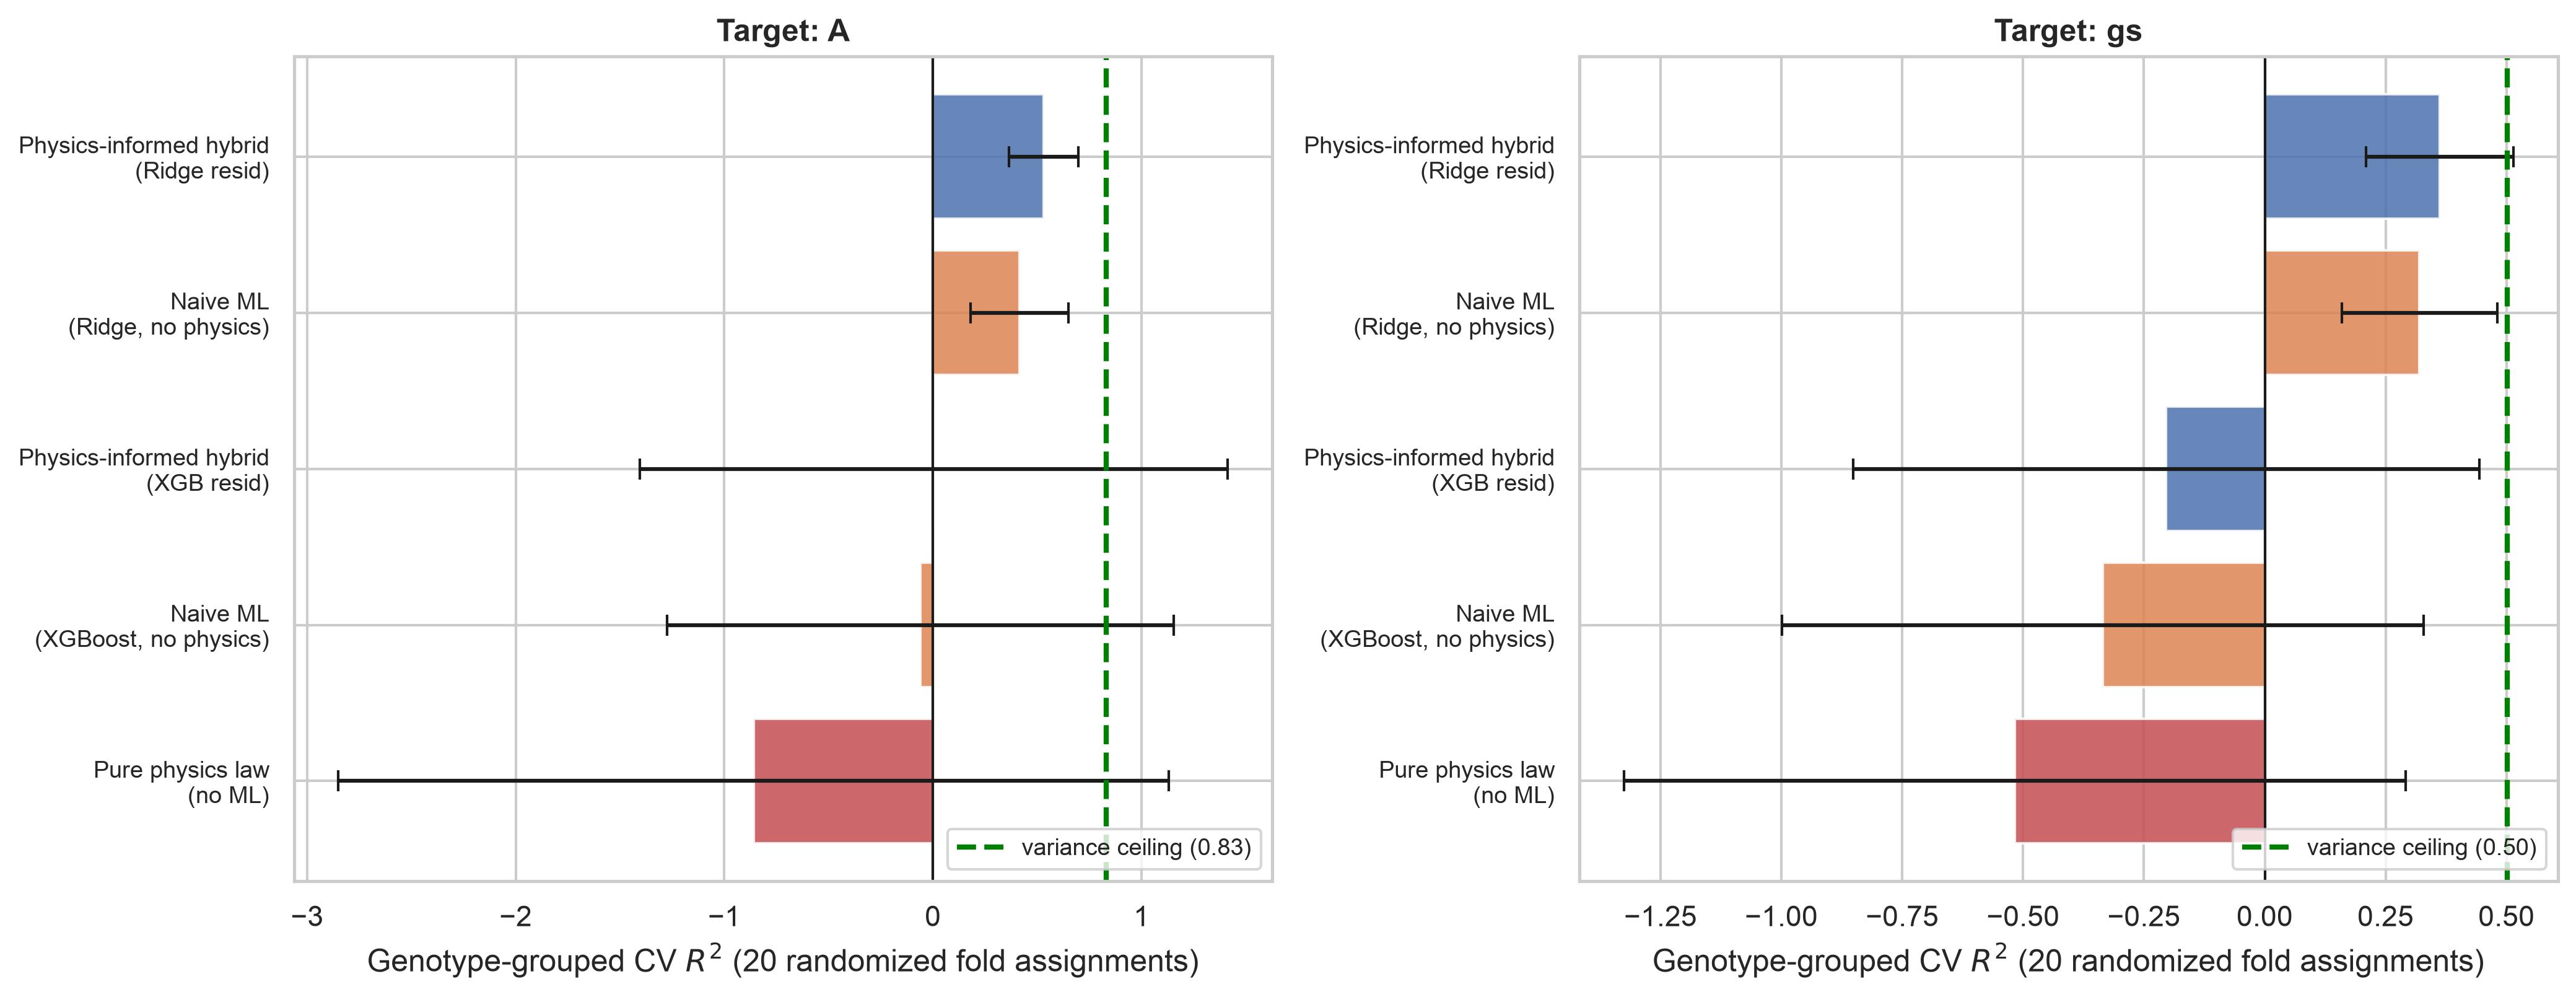
\includegraphics[width=\textwidth]{figures/fig_model_performance.png}
\caption{Genotype-grouped CV $R^{2}$ for all model variants, with error bars over 20 randomized fold assignments. Dashed green lines mark the variance ceiling (Table~\ref{tab:ceiling}).}
\label{fig:modelperf}
\end{figure}

\begin{figure}[t]
\centering
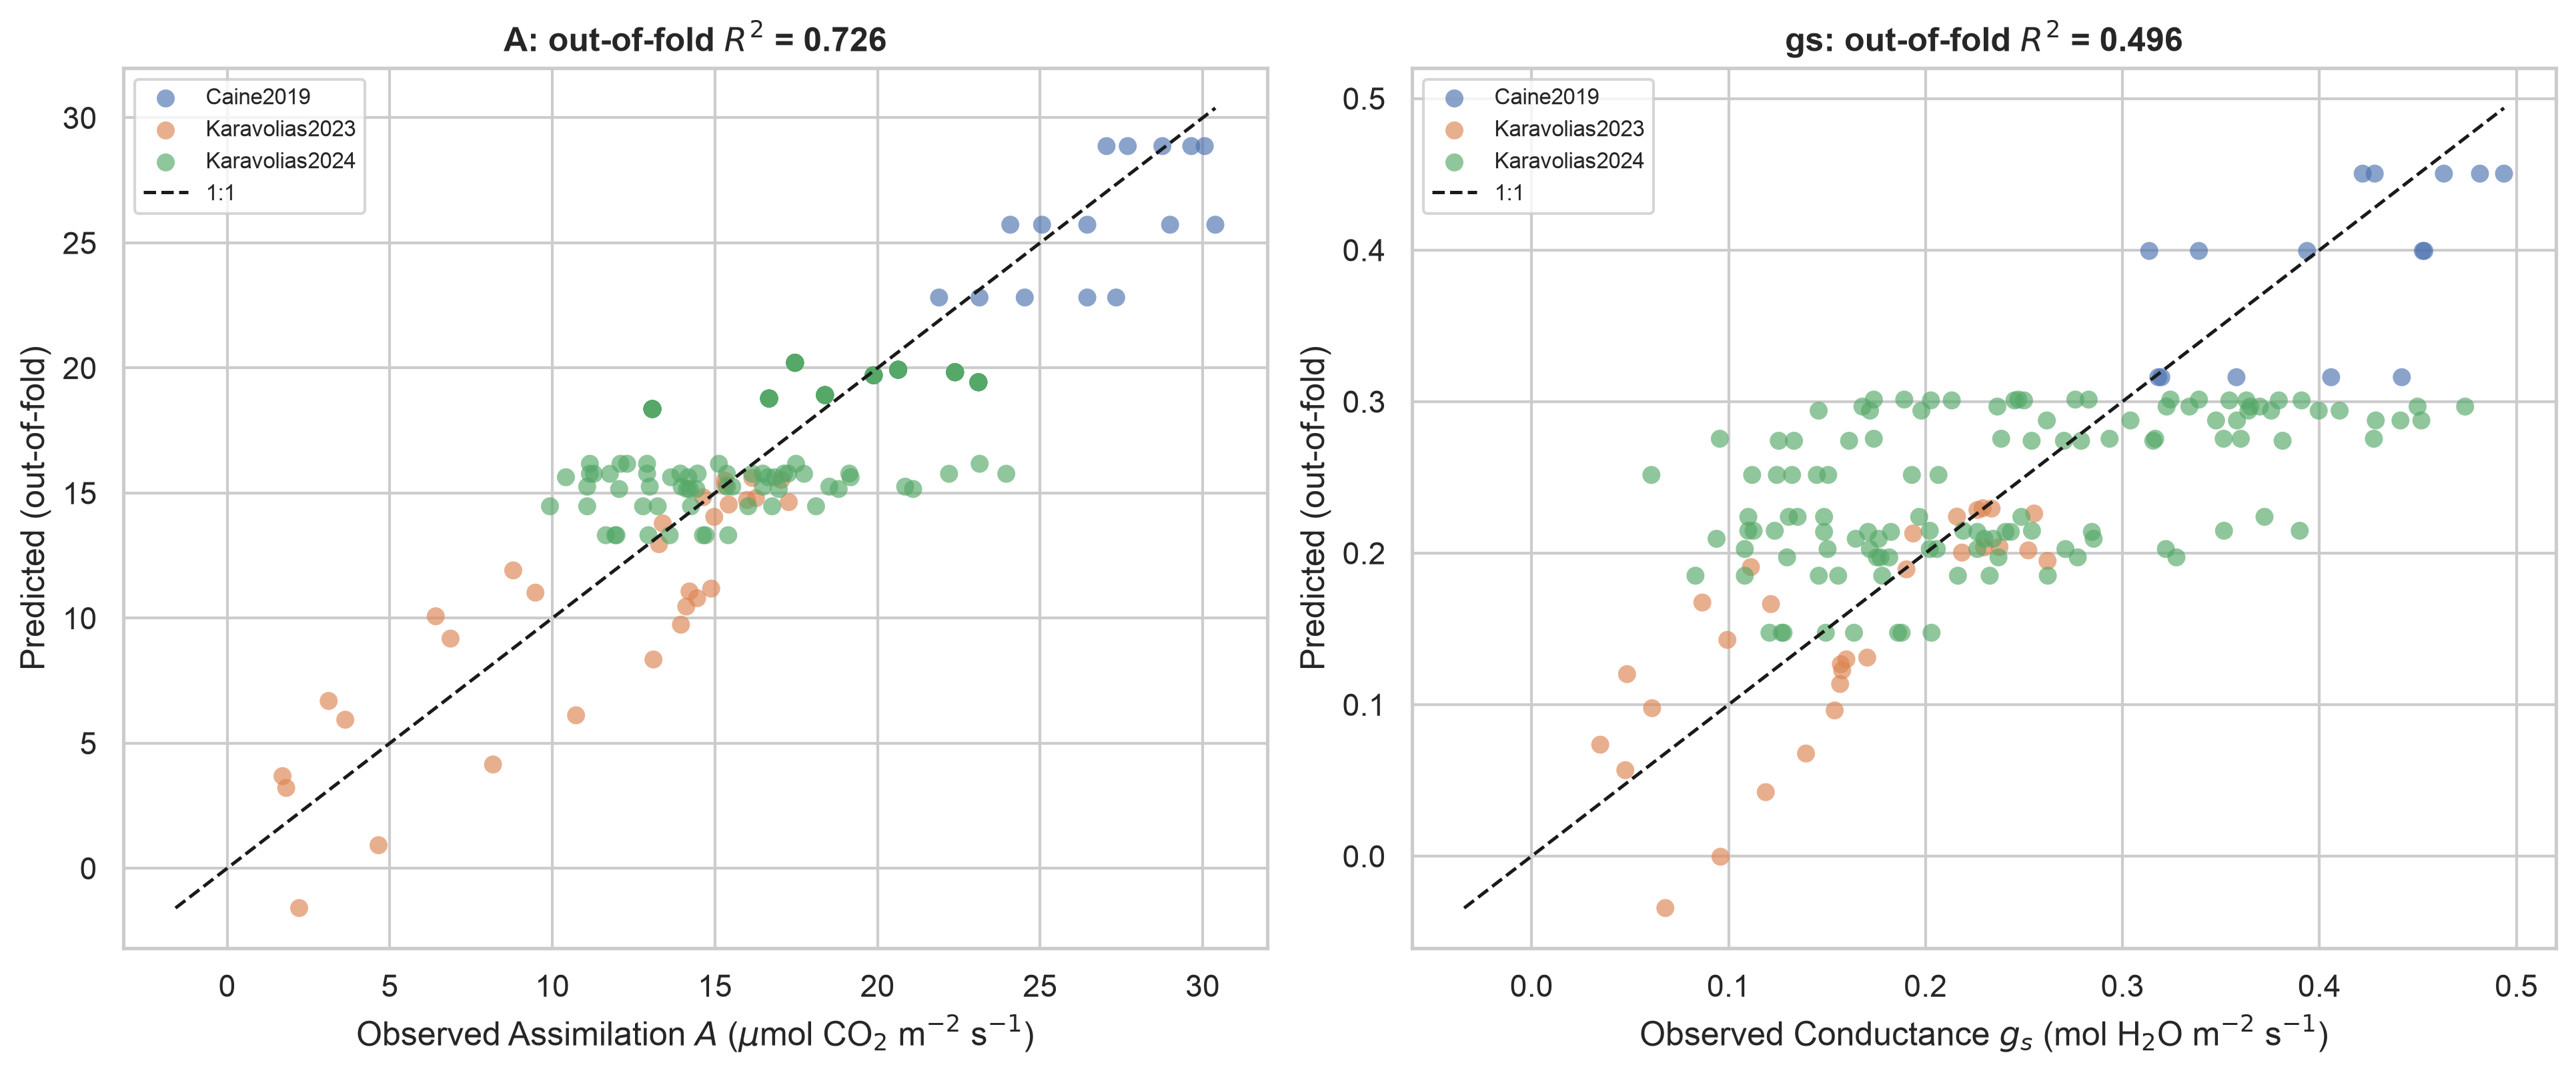
\includegraphics[width=\textwidth]{figures/fig_pred_vs_obs.png}
\caption{Out-of-fold predictions versus observations for assimilation (left) and conductance (right), colored by source study. Dashed line is 1:1.}
\label{fig:predobs}
\end{figure}

The fitted priors are physiologically interpretable:
\begin{align}
A &= 20.51\,\frac{\mathrm{PPFD}}{\mathrm{PPFD}+198}\,S^{0.046}, &
g_s &= 0.291\,\frac{\mathrm{PPFD}}{\mathrm{PPFD}+167}\,S^{0.130}.
\end{align}
Both half-saturation constants (198 and 167\,$\mu$mol\,m$^{-2}$\,s$^{-1}$) fall in the expected range for C3 light-response curves. The density exponents are informative: $\beta_{g_s}=0.130$ is roughly $2.8\times$ $\beta_{A}=0.046$, meaning conductance declines substantially more steeply with density reduction than assimilation does. Both exponents are well below 1, indicating that neither quantity scales proportionally with anatomical pore density -- operating conductance is far less than anatomical maximum conductance, and assimilation is buffered further still by mesophyll demand. This sublinear-but-differential response is the quantitative basis for stomatal engineering, and the model recovers it from data rather than assuming it. Figure~\ref{fig:lightresp} shows the fitted priors against the Karavolias et al. (2023) light-response measurements.

\begin{figure}[t]
\centering
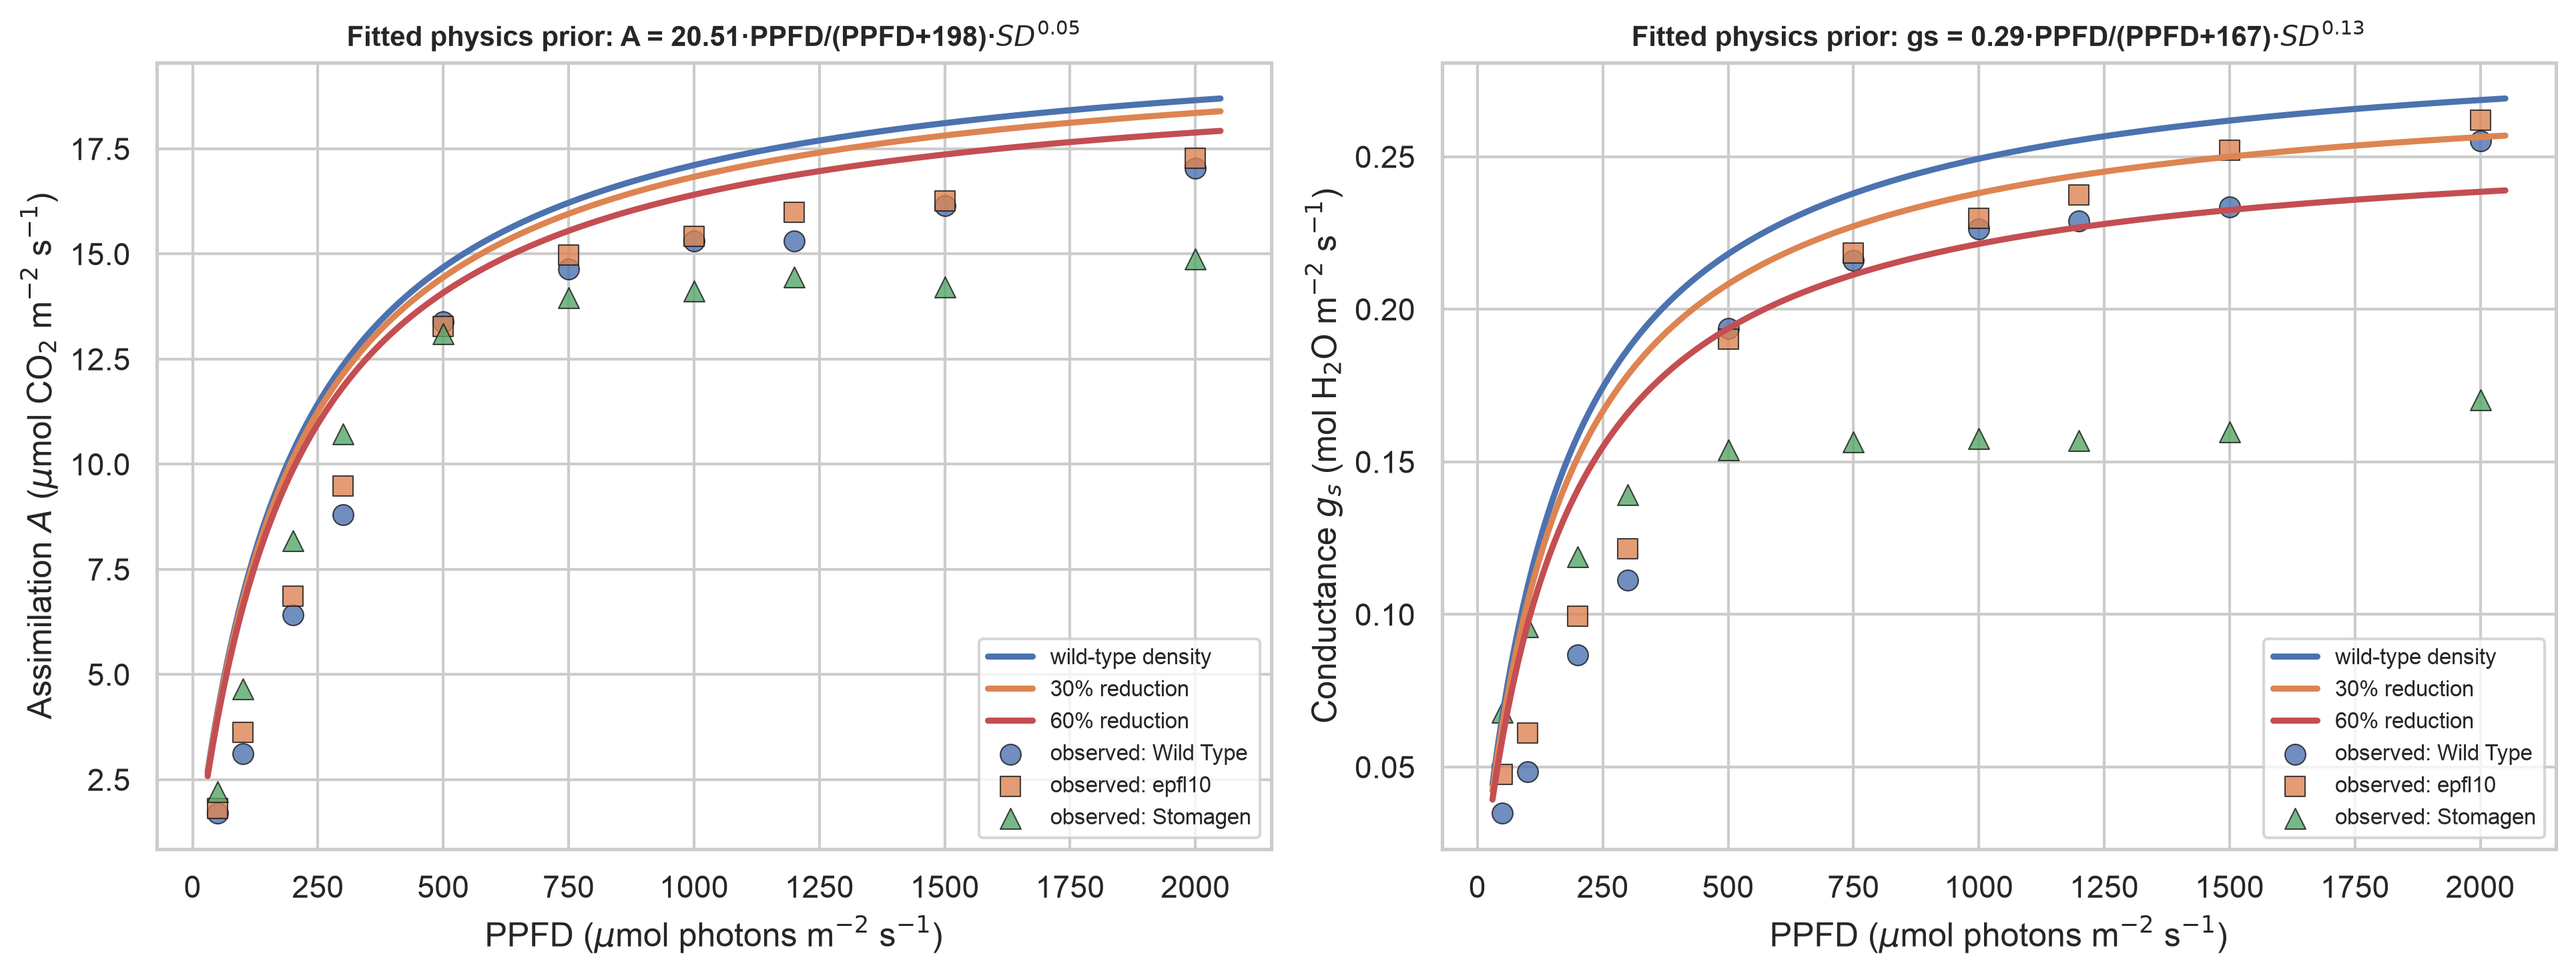
\includegraphics[width=\textwidth]{figures/fig_light_response.png}
\caption{Fitted physics priors (Eq.~\ref{eq:phys}) for assimilation (left) and conductance (right) at three stomatal densities, overlaid on the Karavolias et al. (2023) light-response measurements.}
\label{fig:lightresp}
\end{figure}

\subsection{The Carbon--Water Trade-off}\label{sec:tradeoff}

Because $\beta_{g_s}\gg\beta_{A}$, reducing stomatal density costs proportionally less carbon than the water it saves. Within the validated domain (growth-chamber conditions, PPFD 1500\,$\mu$mol\,m$^{-2}$\,s$^{-1}$, VPD 1.6\,kPa, $29\,^{\circ}$C), the model predicts:

\begin{table}[t]
\caption{Predicted carbon--water trade-off within the validated domain.}\label{tab:tradeoff}
\centering
\small
\begin{tabular}{lcc}
\toprule
\textbf{Density reduction} & \textbf{$A$ retained} & \textbf{$g_s$ retained} \\
\midrule
10\% & 98.3\% & 97.5\% \\
20\% & 96.6\% & 94.8\% \\
30\% & 94.9\% & 92.0\% \\
40\% & 93.1\% & 89.0\% \\
\bottomrule
\end{tabular}
\end{table}

At 30\% reduction the model predicts retention of 94.9\% of wild-type assimilation against 92.0\% of conductance. Figure~\ref{fig:tradeoff} plots both curves, with the unmeasured 40--70\% range shaded. We deliberately do not nominate a single optimal reduction: as Section~\ref{sec:gap} shows, the range in which an optimum would most plausibly lie contains no measurements at all.

\begin{figure}[t]
\centering
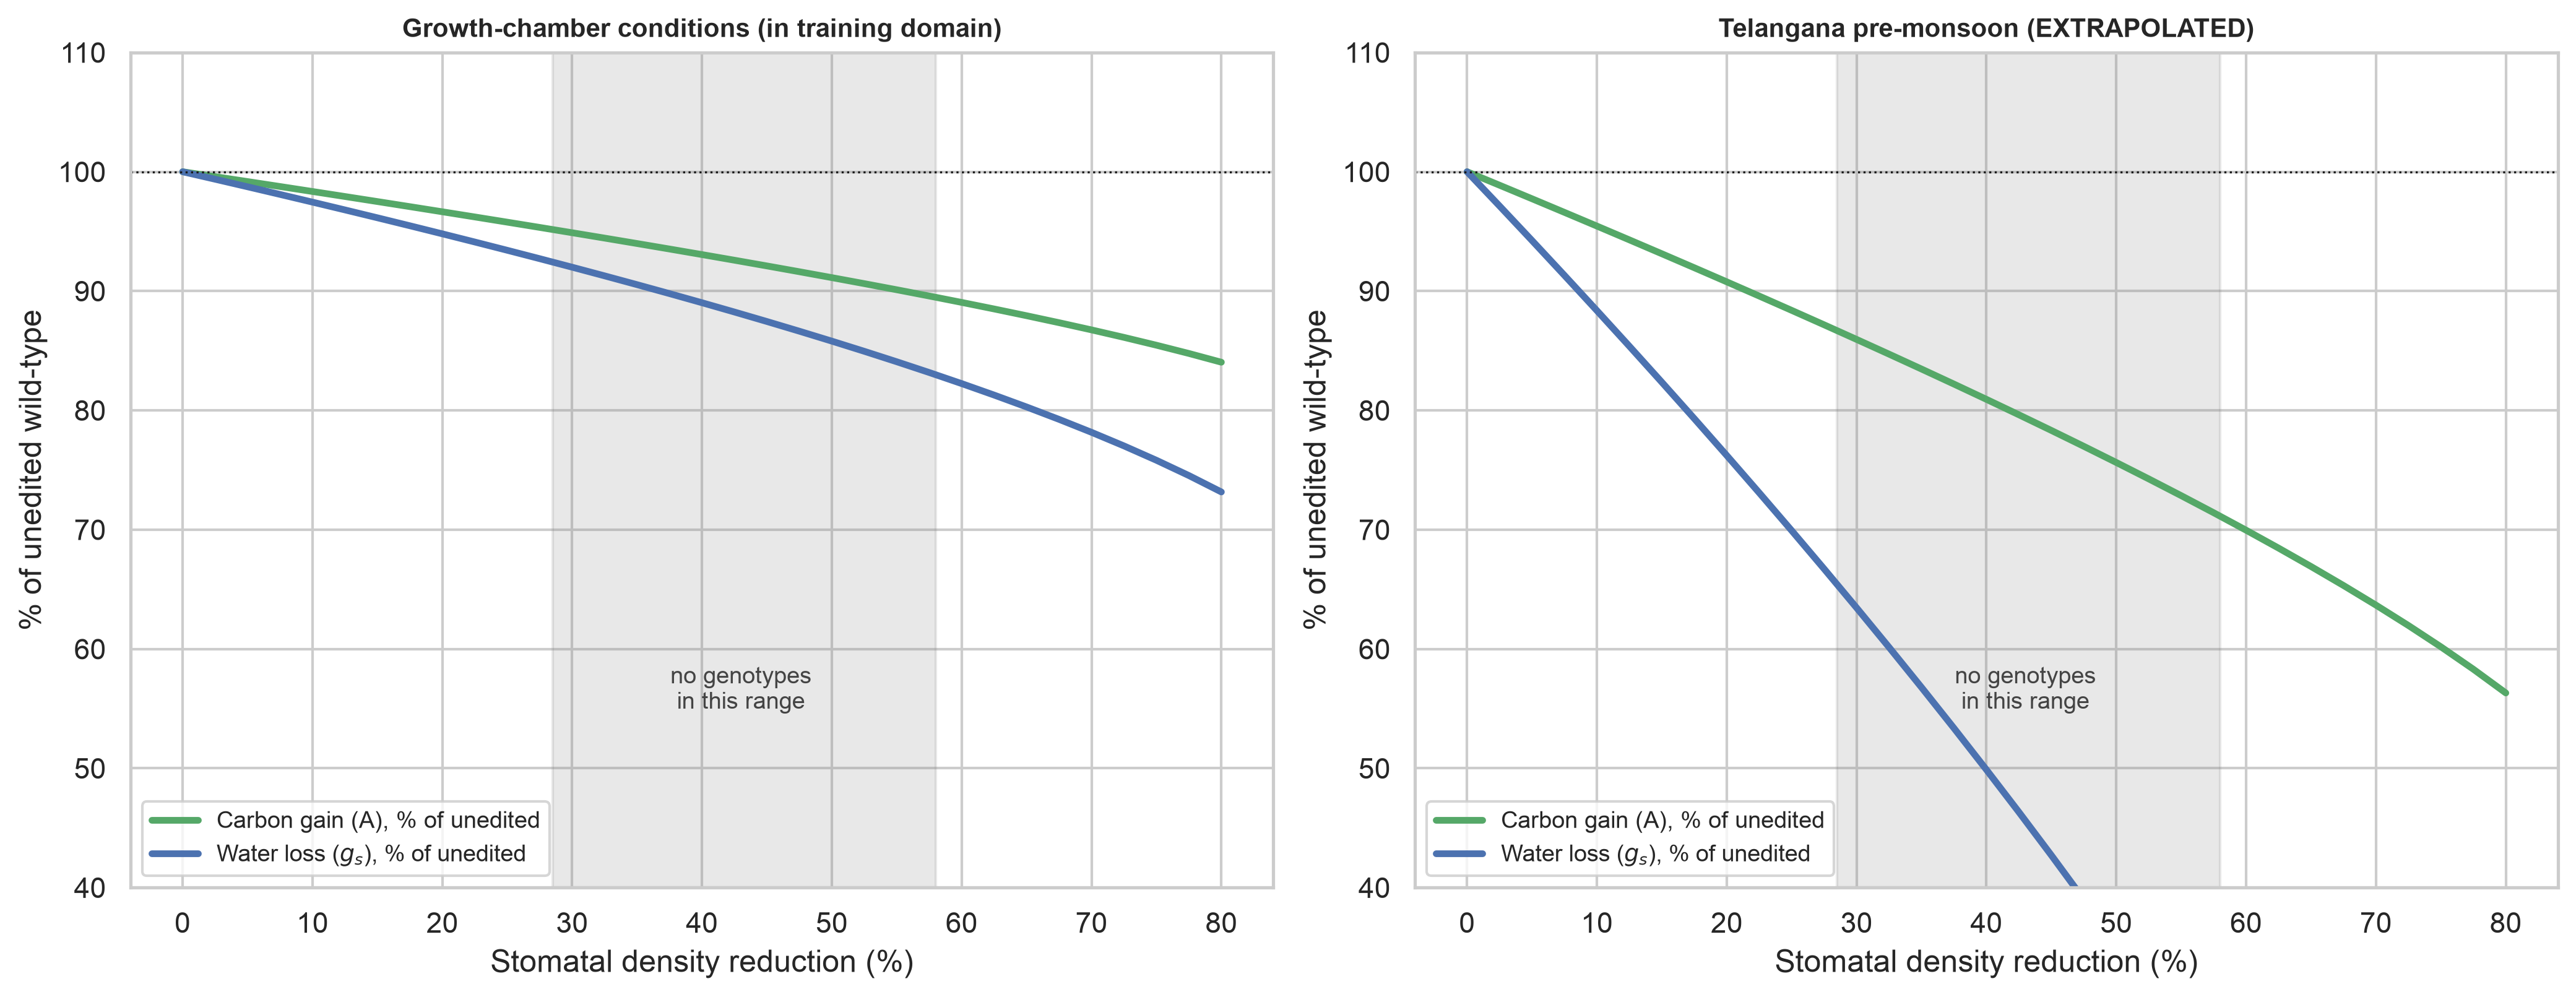
\includegraphics[width=\textwidth]{figures/fig_tradeoff.png}
\caption{Predicted carbon gain and water loss as a function of stomatal density reduction, within the validated domain (left) and extrapolated to Telangana pre-monsoon conditions (right). Shaded band marks the 40--70\% range, where no published measurements exist.}
\label{fig:tradeoff}
\end{figure}

\subsection{Cross-Study Transfer and Domain Limits}\label{sec:transfer}

Leave-one-study-out validation of \emph{absolute} values fails for both targets (assimilation: $R^{2}=-8.20$, $-34.69$, $-1.00$ for held-out Caine, Karavolias 2023 and Karavolias 2024 respectively; conductance: $-3.49$, $-57.15$, $-0.41$). Part of the cause is calibration offset rather than a wrong functional form: wild-type assimilation differs roughly threefold across the three studies (28.6, 11.2 and 20.6\,$\mu$mol\,m$^{-2}$\,s$^{-1}$), reflecting differences in cultivar, instrumentation and growth conditions, and a model trained on two studies has no basis for inferring the absolute level of a third.

We tested whether normalizing each measurement to its own study's wild-type control at matched conditions -- the standard response-ratio device in meta-analysis -- repairs this. It does not. Leave-one-study-out $R^{2}$ on the normalized targets remains negative for both primary quantities ($-0.28$ for $A/A_{\mathrm{WT}}$, $-0.04$ for $g_s/g_{s,\mathrm{WT}}$), with individual folds ranging from $+0.32$ to $-0.96$. Removing the between-study offset therefore removes a real nuisance without exposing a transferable genotype signal underneath. We flag one methodological caution here against our own earlier analysis: an exploratory version of this test using a larger feature set returned weakly \emph{positive} values ($+0.15$ and $+0.07$), and the sign of the result flipped with an arbitrary modelling choice. With three studies, leave-one-study-out estimates rest on three folds and are unstable enough that no configuration-specific value should be trusted; we report the negative result because it is what a pre-specified, minimal feature set gives, and we regard the honest summary as \emph{cross-study transfer is not demonstrated}, rather than either signed estimate.

Separately, all five Telangana district-season scenarios lie outside the training envelope, chiefly in temperature: the source studies were conducted at 28--31$\,^{\circ}$C, whereas district-mean temperatures range from 26.0$\,^{\circ}$C (Kharif) to 33.2$\,^{\circ}$C (pre-monsoon), with VPD reaching 3.39\,kPa against a training maximum of 2.25\,kPa. The right panel of Figure~\ref{fig:tradeoff} is therefore labelled as extrapolation, and field-scale recommendations are deferred pending measurements in that range.

\subsection{Sparse Coverage of the Decision-Relevant Range}\label{sec:gap}

The twelve distinct stomatal-density reduction levels in the combined literature are $-18.0$, $-4.5$, $0$, $4.7$, $9.4$, $12.4$, $16.7$, $28.5$, $58.0$, $78.6$, $78.7$ and $88.0$\%. Coverage is dense below 30\% and again above 78\%, and very thin between: the largest gap between adjacent levels spans 29.5 percentage points, from 28.5\% to 58.0\%, and the entire 30--70\% band -- the range in which a practical design optimum would most plausibly lie -- is represented by a single genotype (\textit{OsEPF1oe}W at 58.0\%, contributing 5 of 165 measurements). This is a property of the published literature, not of our processing. Because the trade-off curves in Figure~\ref{fig:tradeoff} pass through that window supported by one genotype from one study in one cultivar, any optimum identified there would rest almost entirely on the model's functional form rather than on observations, which is why we report the sparsity instead of nominating a target.

\subsection{Reliability Is Not Uniform Across the Reduction Range}\label{sec:genoreliability}

The grouped-CV averages in Table~\ref{tab:perf} combine genotypes of very different reduction magnitude and can mask systematic heterogeneity. We tested this directly with a leave-one-genotype-out analysis: fit on every genotype but one, predict the held-out genotype completely, and repeat for each of the 14 genotype-line groups (Figure~\ref{fig:genoreliability}).

Reliability declines systematically with the magnitude of the engineered change. Across genotypes, leave-one-genotype-out $R^{2}$ correlates negatively with absolute reduction (Spearman $\rho=-0.50$ for $A$, $-0.58$ for $g_s$). Partitioning at the largest data gap, genotypes below 58\% reduction have median $R^{2}$ of $+0.39$ ($A$) and $+0.22$ ($g_s$), whereas the four genotypes at or above 58\% have median $R^{2}$ of $-0.54$ and $-2.24$. The \textit{stomagen} knockout of Karavolias et al. (2024) is the worst case for both targets ($R^{2}=-13.6$ for $A$, $-4.0$ for $g_s$).

Two caveats prevent reading this as a pure severity effect. First, severity is partly confounded with source study: all three Caine et al. lines are predicted poorly (median $R^{2}=-0.61$ for $A$, $-0.49$ for $g_s$, versus $+0.28$ and $+0.22$ for the other two studies) regardless of their reduction level, and that study contributes only 5 measurements per genotype in a cultivar no other study uses. Second, with 14 groups these medians rest on small counts. What the analysis establishes robustly is the negative direction of the relationship and the fact that the aggregate $R^{2}$ in Table~\ref{tab:perf} is carried disproportionately by moderate-reduction genotypes, not that severity alone is the mechanism.

\begin{figure}[t]
\centering
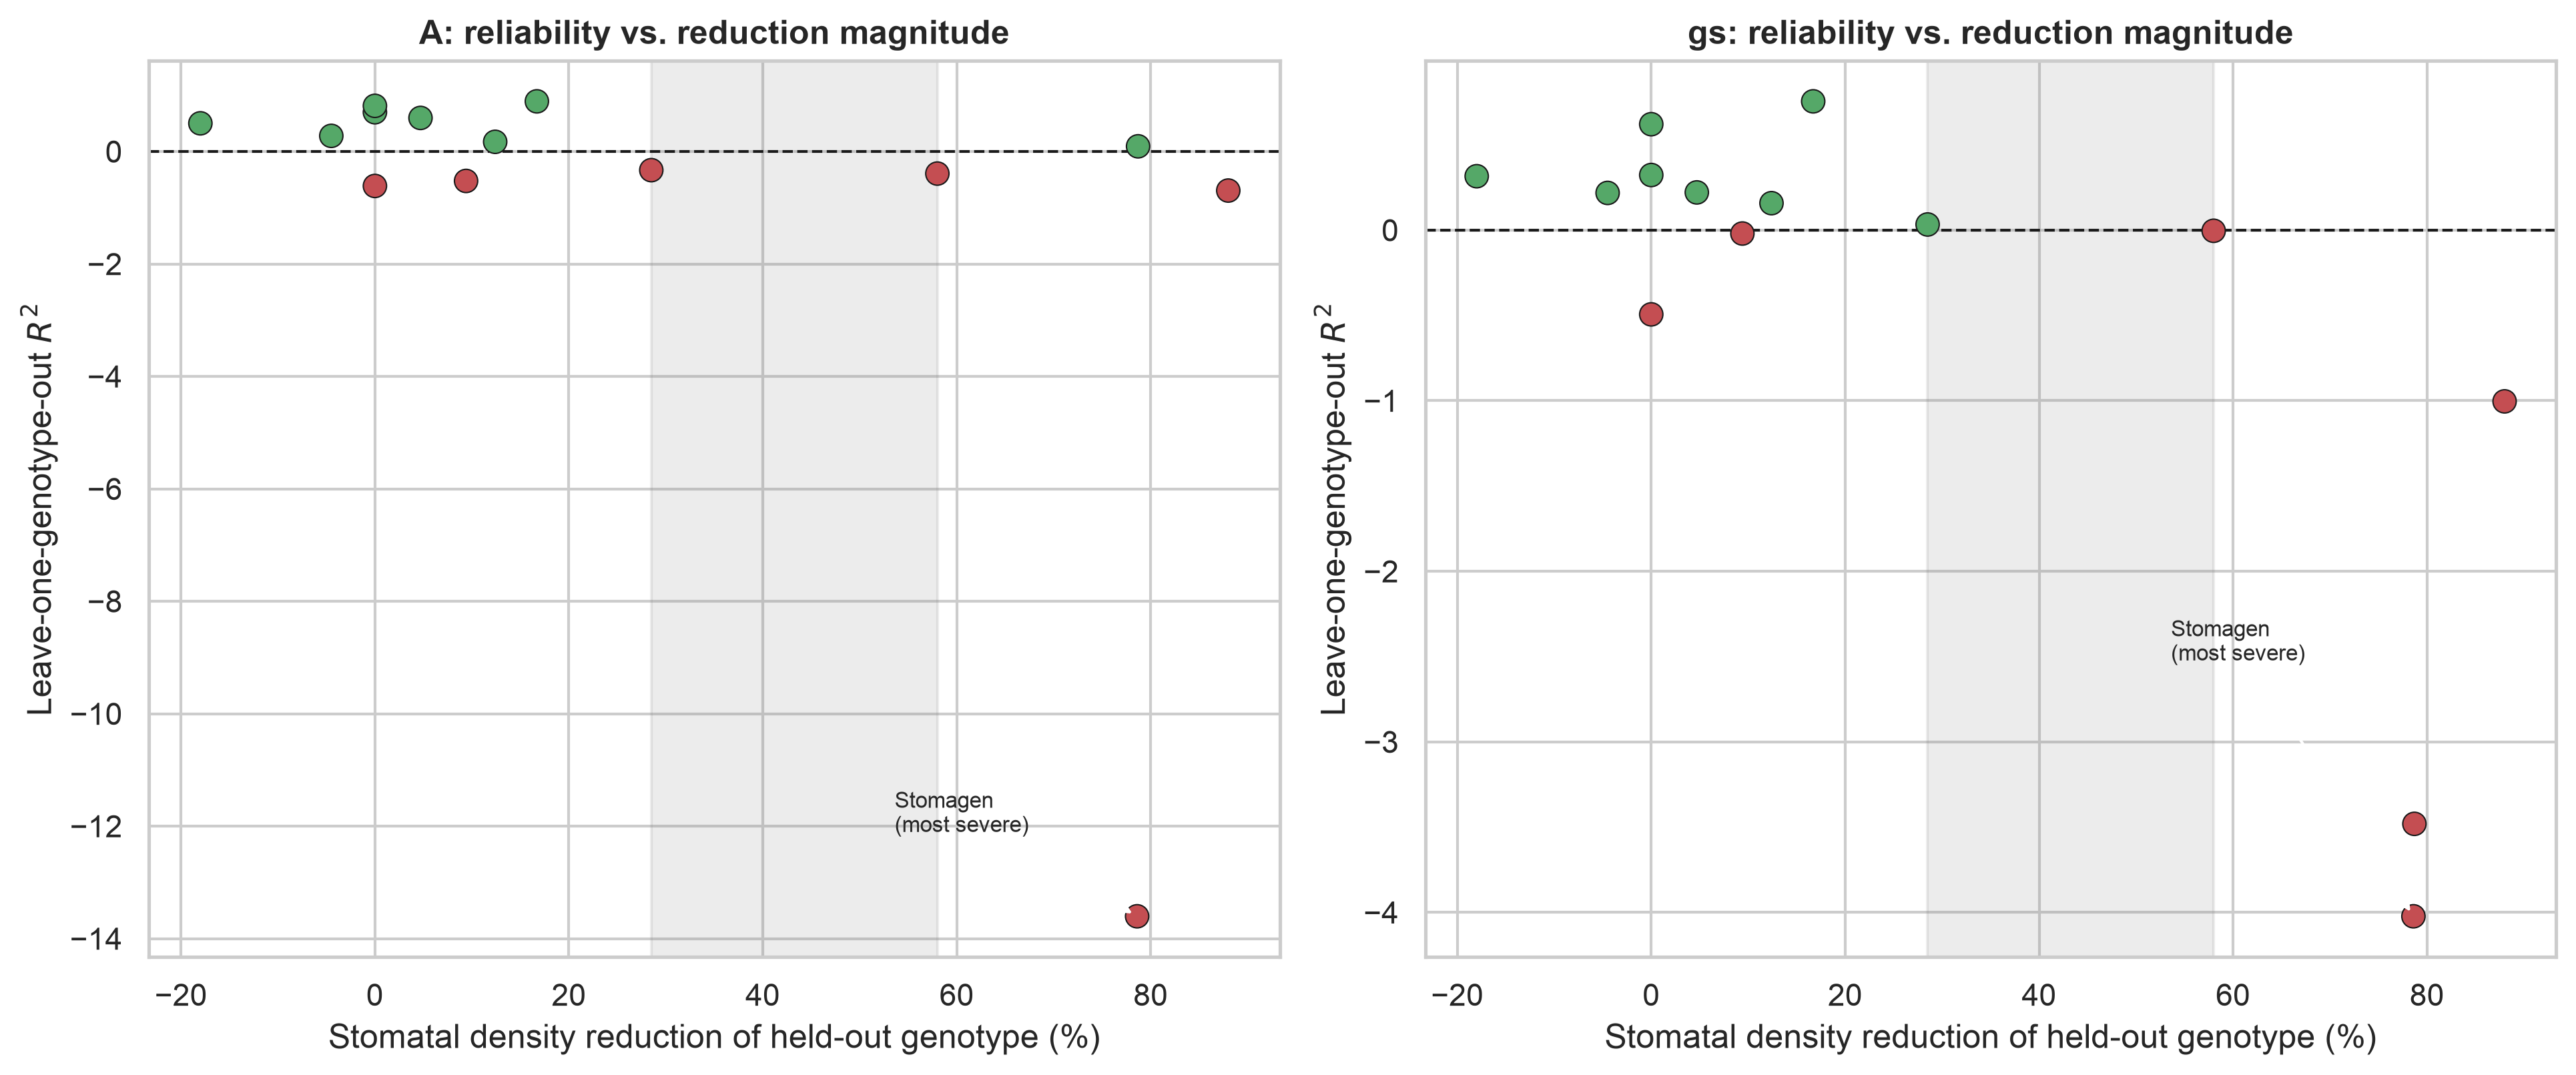
\includegraphics[width=\textwidth]{figures/fig_genotype_reliability.png}
\caption{Leave-one-genotype-out $R^{2}$ versus the held-out genotype's stomatal-density reduction, for $A$ (left) and $g_s$ (right). Red points score below zero. The most severe knockout in the dataset ($\sim$79\% reduction) is the worst-predicted genotype for both targets. Shaded band marks the unmeasured 40--70\% range (Section~\ref{sec:gap}).}
\label{fig:genoreliability}
\end{figure}

The practical consequence is that the trade-off curves in Figure~\ref{fig:tradeoff} should be read with declining confidence as reduction increases, and we regard predictions above roughly 30\% reduction as illustrative rather than validated -- a bound set by where genotype-level validation still succeeds, and which coincides with where the data become sparse (Section~\ref{sec:gap}). More genotypes spanning both the 30--70\% band and the severe tail would be needed to validate that region.

\subsection{Validation Design and Leakage}\label{sec:leakage}

Validation design materially affects reported performance on data of this structure, and we quantify the effect directly. Holding model, target, features and fold count fixed and varying only whether folds respect genotype boundaries, shuffled 5-fold cross-validation inflates $R^{2}$ relative to genotype-grouped cross-validation by $+0.222$ for $A$ ($0.686$ versus $0.464$), $+0.177$ for $g_s$ ($0.491$ versus $0.314$) and $+0.396$ for $A/g_s$ ($-0.001$ versus $-0.397$), averaged over 20 randomized fold assignments (Table~\ref{tab:leakage}). With 14 genotype lines contributing 165 measurements, replicate rows are near-duplicates, so a shuffled split largely measures interpolation between replicates of a genotype the model has already seen rather than generalization to a new genotype. The inflation is largest for the ratio target, which has the least real signal to dilute it. All performance figures reported in this paper are genotype-grouped.

\begin{table}[t]
\caption{Leakage from shuffled cross-validation. Identical model, features and fold count; only the fold-assignment rule differs. Mean over 20 randomized assignments.}\label{tab:leakage}
\centering
\small
\begin{tabular}{lccc}
\toprule
\textbf{Target} & \textbf{Shuffled 5-fold $R^{2}$} & \textbf{Genotype-grouped $R^{2}$} & \textbf{Inflation} \\
\midrule
$A$ (assimilation) & $+0.686$ & $+0.464$ & $+0.222$ \\
$g_s$ (conductance) & $+0.491$ & $+0.314$ & $+0.177$ \\
$A/g_s$ (intrinsic WUE) & $-0.001$ & $-0.397$ & $+0.396$ \\
\bottomrule
\end{tabular}
\end{table}

% ============================================================
\section{Discussion}\label{sec:discussion}

\subsection{Principal Findings}
A physics-informed model combining a saturating light-response prior with a ridge residual predicts assimilation and conductance in stomatal-engineered rice at 64\% and 72\% of their respective ICC-corrected ceilings, using 165 measurements drawn from three heterogeneous studies. The physics prior contributes a reproducible improvement over an identical model without it (20/20 paired repeats for both targets), supporting the central claim motivating PIML in small-data regimes. The fitted density exponents recover the differential sensitivity of conductance and assimilation that makes stomatal engineering viable, and quantify it: $\beta_{g_s}/\beta_A \approx 2.8$, with both exponents well below unity. That aggregate performance is not uniform, however: Section~\ref{sec:genoreliability} shows it is carried by moderate-reduction genotypes and degrades systematically as the engineered change grows more severe.

\subsection{Target Selection Is a Modelling Decision}
The most consequential decision in this work was not architectural but the choice of dependent variable. Intrinsic water-use efficiency is the quantity of primary agronomic interest and the natural target, yet it is unlearnable from data of this kind: its ICC-corrected ceiling is $R^{2}=0.00$, and its between-genotype signal is 2.7$\times$ smaller than replicate scatter. Modelling its two constituents separately -- each with a far higher ceiling -- and reporting the trade-off between them recovers a usable framework. We recommend computing Eq.~\ref{eq:ceiling} for any candidate target before model development, particularly where the target is a ratio, index or other derived quantity, since it costs nothing and bounds what any subsequent effort can achieve; we also recommend using the ANOVA ICC rather than a naive sum-of-squares ratio whenever any replicate group may contain a single observation, since that case is common in small biological datasets and the naive estimator is biased upward exactly then.

\subsection{Model Class in the Small-Sample Regime}
Gradient-boosted trees underperformed ridge regression on every comparison here, often substantially and always with much greater variance. This is a structural consequence of grouped validation: when each genotype contributes a distinct value of the principal continuous predictor, holding one out requires interpolation across that predictor, which piecewise-constant ensembles cannot do. Flexible learners are not automatically preferable where the grouping structure of the data forces interpolation rather than recall.

\subsection{Limitations}\label{sec:limitations}
\begin{enumerate}
    \item \textbf{Reliability degrades with reduction severity.} Leave-one-genotype-out $R^{2}$ correlates negatively with reduction magnitude ($\rho=-0.50$ to $-0.58$), and severity is partly confounded with source study (Section~\ref{sec:genoreliability}). Predictions above roughly 30\% reduction should be treated as illustrative, not validated.
    \item \textbf{Imputed assimilation values.} 59 of 165 rows use regression-estimated rather than measured $A$ ($R^{2}=0.931$ on 8 genotype means). These are flagged in the released data, but they are not independent measurements and will inflate apparent fit for the drought subset.
    \item \textbf{Cross-study transfer is not demonstrated.} Absolute predictions do not transfer, and wild-type normalization does not repair this. Leave-one-study-out estimates rest on three folds and changed sign between two reasonable feature sets, so no signed value from this test is reliable.
    \item \textbf{Extrapolation.} All Telangana scenarios lie outside the training envelope, chiefly in temperature and VPD.
    \item \textbf{Sparse coverage where it matters.} The largest gap between adjacent reduction levels spans 28.5--58.0\%, and the whole 30--70\% band rests on one genotype (5 measurements).
    \item \textbf{Confounding.} Temperature, CO$_2$ and, for two of three studies, VPD are constant within study, so their fitted effects are not cleanly separable from study identity.
    \item \textbf{Hyperparameter selection.} The ridge penalty ($\alpha=1$) was fixed by a sensitivity check across $\alpha\in[0.1,30]$ rather than nested cross-validated tuning; results are qualitatively stable across that range (grouped $R^2$ for $A$: 0.53 at $\alpha=0.1$ to 0.41 at $\alpha=30$) but $\alpha$ was not formally optimized.
    \item \textbf{Scope.} Lab conditions only; stomatal density in isolation, excluding pore size, aperture kinetics and spatial patterning; rice only.
    \item \textbf{Digitization and provenance.} Values read from published figures carry unquantified reading error and no repeat-digitization reliability check was performed. Caine et al. stomatal-density reductions are taken from that paper's Results text rather than digitized, after we found an earlier version of this dataset had used densities inconsistent with the source (39\%/71\% against the stated 58\%/88\%); we recommend such cross-checks against stated values as routine practice when compiling from figures.
    \item \textbf{Selection over modelling choices.} Target variable, model class and feature set were chosen partly by comparing validation scores within this dataset. The ceiling analysis and the 20/20 paired physics result are robust to that process, but the specific $R^{2}$ values carry some selection optimism and should be read as approximate.
\end{enumerate}

\subsection{Future Work}
The most valuable next contribution is experimental rather than computational: genotypes spanning 40--70\% stomatal-density reduction, phenotyped across a temperature and VPD range that overlaps field conditions, with a wild-type control in every environment. Such a dataset would convert the extrapolations in Figure~\ref{fig:tradeoff} into interpolations and permit the optimum this framework currently declines to nominate. On the modelling side, a hierarchical formulation with study-level random effects would use the cross-study structure more efficiently than post-hoc normalization, and coupling validated $A$ and $g_s$ predictions to a canopy or crop-growth model would connect leaf-level trade-offs to season-scale yield and water budgets.

% ============================================================
\section{Conclusion}\label{sec:conclusion}

We developed LeafLens, a physics-informed framework for predicting gas exchange in CRISPR stomatal-engineered rice from 165 harmonized measurements across three studies. Coupling a saturating light-response prior with a ridge residual predicts assimilation at $R^{2}=0.53\pm0.17$ and conductance at $R^{2}=0.36\pm0.15$ under genotype-grouped validation, with the physics prior contributing a reproducible benefit in 20 of 20 paired repeats. An ANOVA intraclass-correlation diagnostic explains why the conventional target, intrinsic water-use efficiency, carries no learnable signal in data of this kind ($R^2$ ceiling $=0.00$) while its constituents do (0.830 and 0.501), and we recommend that diagnostic as a routine pre-modelling step for derived targets, particularly given how easily naive variance-ratio estimates are biased by singleton replicate cells. Within its validated domain -- moderate reduction under growth-chamber conditions -- the model predicts that a 30\% density reduction retains 94.9\% of wild-type assimilation against 92.0\% of conductance. We do not extend that prediction further, for three reasons we quantify rather than assert: predictive skill declines as the engineered reduction grows more severe, cross-study transfer is not demonstrated even after wild-type normalization, and the 30--70\% band where a practical optimum would lie is represented in the entire published literature by a single genotype. Filling that band experimentally, with wild-type controls in every environment, would do more to enable rational stomatal design than any further modelling of the data that currently exist.

% ============================================================
\section*{Acknowledgments}
The authors thank the developers of the NASA POWER API for open-access climate data. Source code and data are available at \url{https://github.com/3rishna/LeafLens}.

\section*{Declarations}
\textbf{Funding:} Not applicable. \\
\textbf{Conflict of interest:} The authors declare no competing interests. \\
\textbf{Data availability:} All digitized data, processing scripts and outputs are available at the repository above. \\
\textbf{Use of AI assistance:} An AI coding assistant (Claude, Anthropic) was used for code debugging, pipeline re-verification and manuscript editing. All scientific claims and conclusions were reviewed and are the responsibility of the authors, consistent with Springer Nature policy on AI tools in the writing process.

% ============================================================
\begin{thebibliography}{20}

\bibitem{ref_fao}
FAO: Rice Market Monitor. Food and Agriculture Organization of the United Nations, Rome (2023)

\bibitem{ref_ipcc}
IPCC: Climate Change 2023: Synthesis Report. Intergovernmental Panel on Climate Change, Geneva (2023)

\bibitem{ref_crispr_review}
Zhu, H., Li, C., Gao, C.: Applications of CRISPR--Cas in agriculture and plant biotechnology. Nature Reviews Molecular Cell Biology \textbf{21}(11), 661--677 (2020)

\bibitem{ref_hepworth}
Hepworth, C., Doheny-Adams, T., Hunt, L., Cameron, S.E., Gray, J.E.: Manipulating stomatal density enhances drought tolerance without deleteriously affecting yield. New Phytologist \textbf{207}(4), 1080--1089 (2015)

\bibitem{ref_caine}
Caine, R.S., Yin, X., Sloan, J., Harrison, E.L., Mohammed, U., Fulton, T., Biswal, A.K., et al.: Rice with reduced stomatal density conserves water and has improved drought tolerance under future climate conditions. New Phytologist \textbf{221}(1), 371--384 (2019)

\bibitem{ref_kara2023}
Karavolias, N.G., Patel-Tupper, D., Seong, K., Tjahjadi, M., Gueorguieva, G.-A., Tanaka, J., Gallegos Cruz, A., et al.: Paralog editing tunes rice stomatal density to maintain photosynthesis and improve drought tolerance. Plant Physiology \textbf{192}(2), 1168--1182 (2023)

\bibitem{ref_kara2024}
Karavolias, N.G., Patel-Tupper, D., Gallegos Cruz, A., Litvak, L., Lieberman, S.E., Tjahjadi, M., Niyogi, K.K., Cho, M.-J., Staskawicz, B.J.: Engineering quantitative stomatal trait variation and local adaptation potential by cis-regulatory editing. Plant Biotechnology Journal \textbf{22}, 3442--3452 (2024)

\bibitem{ref_ball_berry}
Ball, J.T., Woodrow, I.E., Berry, J.A.: A model predicting stomatal conductance and its contribution to the control of photosynthesis under different environmental conditions. In: Progress in Photosynthesis Research, pp.~221--224. Springer, Dordrecht (1987)

\bibitem{ref_medlyn}
Medlyn, B.E., Duursma, R.A., Eamus, D., Ellsworth, D.S., Prentice, I.C., Barton, C.V.M., Crous, K.Y., De Angelis, P., Freeman, M., Wingate, L.: Reconciling the optimal and empirical approaches to modelling stomatal conductance. Global Change Biology \textbf{17}(6), 2134--2144 (2011)

\bibitem{ref_karniadakis}
Karniadakis, G.E., Kevrekidis, I.G., Lu, L., Perdikaris, P., Wang, S., Yang, L.: Physics-informed machine learning. Nature Reviews Physics \textbf{3}, 422--440 (2021)

\bibitem{ref_willard}
Willard, J., Jia, X., Xu, S., Steinbach, M., Kumar, V.: Integrating scientific knowledge with machine learning for engineering and environmental systems. ACM Computing Surveys \textbf{55}(4), 1--37 (2022)

\bibitem{ref_ml_agri}
Liakos, K.G., Busato, P., Moshou, D., Pearson, S., Bochtis, D.: Machine learning in agriculture: A review. Sensors \textbf{18}(8), 2674 (2018)

\bibitem{ref_nasa}
NASA Langley Research Center: POWER -- Prediction of Worldwide Energy Resources. \url{https://power.larc.nasa.gov/} (2026)

\bibitem{ref_fao56}
Allen, R.G., Pereira, L.S., Raes, D., Smith, M.: Crop Evapotranspiration -- Guidelines for Computing Crop Water Requirements. FAO Irrigation and Drainage Paper 56. Food and Agriculture Organization, Rome (1998)

\bibitem{ref_mccree}
McCree, K.J.: Test of current definitions of photosynthetically active radiation against leaf photosynthesis data. Agricultural Meteorology \textbf{10}, 443--453 (1972)

\bibitem{ref_searle}
Searle, S.R., Casella, G., McCulloch, C.E.: Variance Components. John Wiley \& Sons, New York (1992)

\end{thebibliography}

\end{document}
